 % LaTeX (version 2e) source for Optimask Documentation
 % IF USE CHINESE Language PACKAGES, THEN MUST USE XeLaTeX to COMPILE !!!
 % Ref.: \OptiXera\Develop\Docs\LaTeX, or \OptiXera\Develop\optixera\optimask\dev\LaTeX\
 % by hdeng@optixera.com
% Created: 2016-12-17; Updated: 2017-05-15;

%======================================================================
%   P R E A M B L E
%======================================================================

%%THIS for pdf Latex with .pdf figures%%%%%%%%%%%%%%

% memoir style %Books split into Volumns
%\documentclass[12pt,twoside]{book}
\documentclass[10pt,twoside]{book}
%\documentclass[journal,twoside]{IEEEtran}

%\documentclass[pdftex]{report}
\usepackage{ifpdf}
\ifpdf
\usepackage[pdftex]{graphicx}
\else
\usepackage[dvips]{graphicx}
\fi
%%%%%%%%%%%%%%%%%%%%%%%%%%%%%%%%%%%%%%%%%%%%%%%

%\usepackage{watermark}; %\usepackage{everypage}; %\usepackage{draftwatermark}; %\usepackage{ncccropmark}

\usepackage{fancyhdr} %fancy headings
\usepackage{amsmath}
\usepackage{cite}
\usepackage{notoccite} %Prevent erroneous numbering of cites when using BibTeX/unsrt
%\usepackage[dvips=true,bookmarks=true]{hyperref} %only needed for PDF generation
%\usepackage{makeidx} %if need an index
\usepackage[printonlyused]{acronym} %\usepackage{acronym} %if need list of acronyms
%\usepackage{nomencl}
%\usepackage{stfloats}
%\usepackage{float}
\usepackage{subfigure}
%\usepackage{array}
%\usepackage{psfrag}
\usepackage{color}
\usepackage{listings} %for showing program codes
%\usepackage[normalem]{ulem}  %to underline serveral lines; NO underline for \emph{}!!

%Custom packages:
%\usepackage[first]{datestamp} %first, all, off.
\usepackage[all]{datestamp}
%Datestamp on first page of each chapter
%\usepackage{glosstex} %preparation of glossaries, lists of acronyms or sorted lists in general


%Show Line Numbers at the left side of the page
\usepackage{lineno} %for single column articles
%\usepackage[switch]{lineno} %for double column articles
\linenumbers

% *** CHINESE Language PACKAGES (Select One of These Methods)***
%% !! MUST USE XeLaTeX to COMPILE !!! OTHERWISE, WILL HAVE ERROR!
%
%% Method 1: Refer to testXeTeX.tex, use XeLaTex+fontspec package
%\usepackage{fontspec, xunicode, xltxtra}
%\XeTeXlinebreaklocale "zh"
%\XeTeXlinebreakskip = 0pt plus 1pt minus 0.1pt
%\setmainfont{SimSun} %新宋体 %{FZShuTi}字体不存在,用{FZShuTi}字体编译出错。
% 
%\setmainfont{Times}
%
%% Method 2: Refer to testXeCJK.tex, use XeLaTex+XeCJK package
\usepackage{xeCJK} % 调用 xeCJK 宏包
\setCJKmainfont{SimSun} % 设置 CJK 主字体为 SimSun (宋体)
%TeX default font: Computer Modern Roman, size: 10pt.

%----------------------------------------------------------------------
%\makeindex % activate index-making
%\makeglossary %activate nomencl (list of symbols) making

%----------------------------------------------------------------------
% Set "1.2" as the line spacing throughout the thesis for readability (optional).
\renewcommand{\baselinestretch}{1.2}

%----------------------------------------------------------------------
% Reset page margins properly (commented is for doublesided pages)
\setlength{\marginparwidth}{0pt}
\setlength{\marginparsep}{0pt}
\setlength{\oddsidemargin}{0.125in}
\setlength{\evensidemargin}{0.125in}
\setlength{\textwidth}{6.375in}
\raggedbottom
%----------------------------------------------------------------------
%My own command & environment definitions (More in course.tex of Waterloo's source.zip):
%Some Latin abbreviations in italic (\MakeLowercase{\textit{et al.}}; space after "\" produces a space):
\newcommand{\eg}{\textit{e.g.}}      %e.g. = exempli gratia = for example
\newcommand{\ie}{\textit{i.e.}}      %i.e. = id est = that is
\newcommand{\cf}{\textit{c.f.}}      %c.f. = confer = compare
\newcommand{\etc}{\textit{etc}.\@}    %etc = et cetera = and the rest
\newcommand{\etal}{\textit{et~al}.\@} %et al = et alia = and other
%\newcommand{\degree}{^\circ}


%%Define own words
 \def\InP{$\mathrm{InP}$}
 \def\InGaAsP{$\mathrm{InGaAsP}$}
 \def\InGaAsPxy{$\mathrm{In_{1-x}Ga_{x}As_{y}P_{1-y}}$}
 \def\um{$\mu\mathrm{m}$}
 \def\nm{$\mathrm{nm}$}

%----------------------------------------------------------------------
%%%to include subsubsections in the table of contents
%%%%%\renewcommand*\thesubsubsection{\Roman{subsubsection}.} %\arabic{},\alph{},\roman{},\Alph{},\Roman{}
\setcounter{secnumdepth}{3} %%add numbering depth
\setcounter{tocdepth}{3}

%======================================================================
%   L O G I C A L    D O C U M E N T
%======================================================================
\begin{document}

%----------------------------------------------------------------------
% FRONT MATERIAL
%----------------------------------------------------------------------
% TITLE PAGEs (may need to space and format this page yourself)
% By Henghua DENG; Created: 2009-11-20; Updated: 2009-11-20;

\pagestyle{empty} % No headers or page numbers

\begin{center}

\vspace*{1.0cm} \Huge{Optimask Manual}

\vspace*{1.0cm}
\normalsize
by \\
\vspace*{1.0cm}
\Large
Optixera\\
\vspace*{2.0cm}
\normalsize
Optixera \\
USA and China\\


\vspace*{2.0cm} Silicon Valley, California, USA, \the\year\\ %\the\year, %\today
%\vspace*{2.0cm} Silicon Valley, California, USA, 2012\\

\vspace*{2.0cm} \copyright Optixera \the\year\\
\end{center}

\newpage

%%%%%%%%%%%%%%%%%%%%%%%%%%%%%%%%%%%%%%%%%%%%%%%%%%%%%%%%%%%%%
% PRELIMINARY PAGES
%%%%%%%%%%%%%%%%%%%%%%%%%%%%%%%%%%%%%%%%%%%%%%%%%%%%%%%%%%%%%
\pagestyle{plain} % No headers, just page numbers
\pagenumbering{roman} % Roman numerals
\setcounter{page}{2}

%% Declaration Page for ELECTRONIC SUBMISSION OF A THESIS
%\begin{center}\large \textbf{Author's Declaration For Electronic Submission} \end{center}
%\noindent I hereby declare that I am the sole author of this report. \\

%\noindent I understand that my thesis may be made electronically
%available to the public. \vspace{4cm}

%\noindent Henghua Deng
%\newpage

% Long abstract (manually formatted)
\resetdatestamp %Date Stamp--Only use when custom package datestamp.sty is used.
\begin{center}\Large \textbf{Abstract} \end{center}
\addcontentsline{toc}{chapter}{Abstract}
Optimask is a revolutionary layout tool for advanced photomask drawing. It is developed after decades of professional experience from elite engineers and researchers in semiconductor and photonics industry companies, as well as scientific institutes and universities. Our team of international developers consist of photonic experts, electronics researchers and computer scientists. Our primary and ultimate goal is to simplify photonics simulation and photomask design as easy as word processing, with increased accuracy, precision, versatility, and portability. We will make photomask drawing a pleasure, and remove the barrier of advanced knowledge, skill-set and training required.

\vspace*{1em} %\textbf{Index Terms:}
\begin{description}
    \item[\emph{Index Terms}:]
      \small{\acf{GDSII}}
\end{description}
\newpage

% Acknowledgements and/or Dedication Pages
\begin{center}\Large \textbf{Acknowledgements}\end{center}
\addcontentsline{toc}{chapter}{Acknowledgements}

We would like to express our sincere gratitude to all people who helped with this product.

\begin{flushright}
Optixera \\ 10/22/2007--\today \\
Revised: \today \\
\end{flushright}

\newpage

% Pages which are generated automatically
%%\setcounter{page}{6} % Set this counter to get correct page numbers
\tableofcontents
\listoftables
\addcontentsline{toc}{chapter}{List of Tables}
\listoffigures
\addcontentsline{toc}{chapter}{List of Figures}
\newpage

% Pages of List of Acronyms

\chapter*{List of Acronyms}
%Chapter style and no numbering, not included in the Table of Contents (TOC)
%For smaller fonts: \begin{center} \Large \textbf{List of Acronyms} \end{center}

%\ac{}--General Form. To enter an acronym inside the text.
%       The first time you use an acronym, the full name of the acronym along
%       with the acronym in brackets will be printed.
%\acf{}--To get Full Name (full version) of the acronym.
%\acs{}--To get the short version of the acronym.
%\acl{}--To get the expanded acronym without mentioning the acronym
%\acp{}, \acfp{}, \acsp{}, aclp{}--plural form of \ac{}, \acf{}, \acs{}, acl{}
%
\begin{acronym}[ATGONUPIC]
 \acro{2D}{two-dimensional}
 \acro{3D}{three-dimensional}
 \acro{AES}{Auger Electron Spectroscopy}
 \acro{AFM}{Atomic Force Microscopy}
 \acro{AON}{All Optical Network}
 \acro{APD}{Avalanche Photodiode}
 \acro{ASIC}{Application Specific Integrated Circuit}
 \acro{ATG}{Asymmetric Twin-Waveguide}
 \acro{ATR}{Attenuated Total Reflection}
 \acro{AWG}{Arrayed Waveguide Grating}
 \acro{BPM}{Beam Propagation Method}
 \acro{BPD}{Balanced Photo-Detectors}
 \acro{CMT}{Coupled Mode Theory}
 \acro{CMOS}{Complementary Metal Oxide Semiconductor}
 \acro{CROW}{Coupled Resonator Optical Waveguide}
 \acro{CVD}{Chemical Vapor Deposition}
 \acro{dB}{decibel}
 \acro{DBR}{Distributed Bragg Reflector}
 \acro{DFB}{Distributed-Feedback}
 \acro{d.f.}{Degrees of Freedom}
 \acro{DQPSK}{Differential Quadrature Phase Shift Keying}
 \acro{DSP}{Digital Signal Processing}
 \acro{DUT}{Device Under Test}
 \acro{DVT}{Design Verification Test}
 \acro{DWDM}{Dense Wavelength Division Multiplexing}
 \acro{EA}{Evolutionary Algorithm}
 \acro{EC}{Evolutionary Computation}
 \acro{EDS}{Energy dispersive x-ray spectroscopy}
 \acro{EIM}{Effective Index Method}
 \acro{EMT}{Effective Medium Theory}
 \acro{EPON}{Ethernet PON}
 \acro{ER}{Extinction Ratio}
 \acro{FD}{Finite-Difference}
 \acro{FDM}{Finite Difference Method}
 \acro{FDTD}{Finite-Difference Time-Domain method}
 \acro{FDTD-BPM}{Finite-Difference Time-Domain Beam-Propagation Method}
 \acro{FD-BPM}{Finite-Difference Beam-Propagation Method}
 \acro{FE}{Finite-Element}
 \acro{FEA}{Finite Element Analysis}
 \acro{FEM}{Finite Element Method}
 \acro{FETD-BPM}{Finite-Element Time-Domain Beam-Propagation Method}
 \acro{FE-BPM}{Finite-Element Beam-Propagation Method}
 \acro{FFT-BPM}{Fast-Fourier-Transform Beam-Propagation Method}
 \acro{FP}{Fabry-Perot}
 \acro{FTTH}{Fiber-To-The-Home}
 \acro{FTTP}{Fiber-To-The-Premises}
 \acro{FV}{Full Vectorial}
 \acro{FWHM}{Full Width at Half Maximum}
 \acro{GA}{Genetic Algorithm}
 \acro{GDSII}{Graphic Data System II}
 \acro{GPON}{Gigabit PON}
 \acro{ID-BPM}{Imaginary-Distance Beam-Propagation Method}
 \acro{IC}{Integrated Circuit}
 \acro{ITU-T}{International Telecommunications Union Telecommunication Standardization Sector}
 \acro{MBE}{Molecular Beam Epitaxy}
 \acro{MEMS}{Micro Electro Mechanical System}
 \acro{MFD}{Mode Field Diameter}
 \acro{MGVI}{Multi-Grid Vertical Integration}
 \acro{MMI}{Multi-Mode Interferometer}
 \acro{MQW}{Multiple Quantum Well}
 \acro{MZDI}{Mach-Zehnder Delay Interferometer}
 \acro{MZI}{Mach-Zehnder Interferometer}
 \acro{MZM}{Mach-Zehnder Modulator}
 \acro{OADM}{Optical Add-Drop Multiplexer}
 \acro{OEIC}{Optoelectronic Integrated Circuit}
 \acro{OLT}{Optical Line Terminal}
 \acro{OMT}{Optical Modal Transformer}
 \acro{ONU}{Optical Network Unit}
 \acro{OPAD}{Optically Pre-Amplified Detector}
 \acro{PARC}{Passive Active Resonant Coupler}
 \acro{PBG}{Photonic Bandgap device}
 \acro{PhC}{Photonic Crystal}
 \acro{PCF}{Photonic Crystal Fiber}
 \acro{PCW}{Photonic Crystal Waveguide}
 \acro{PCM}{Process Control Monitor}
 \acro{PECVD}{Plasma Enhanced Chemical Vapor Deposition}
 \acro{PD}{Photodetector}
 \acro{PDL}{Polarization Dependent Loss}
 \acro{PIC}{Photonic Integrated Circuit}
 \acro{PLC}{Planar Lightwave Circuit}
 \acro{PMD}{Polarization Mode Dispersion}
 \acro{PML}{Perfectly Matched Layer}
 \acro{PON}{Passive Optical Network}
 \acro{QAM}{Quadrature Amplitude Modulation}
 \acro{QWI}{Quantum Well Intermixing}
 \acro{QPSK}{Quadrature Phase Shift Keying}
 \acro{RIE}{Reactive Ion Etching}
 \acro{ROADM}{Reconfigurable Optical Add-Drop Multiplexer}
 \acro{RMS}{Root Mean Square}
 \acro{SAG}{Selective-Area Growth}
 \acro{SEM}{Scanning Electron Microscope}
 \acro{SMF}{Single-Mode Fiber}
 \acro{SOA}{Semiconductor Optical Amplifier}
 \acro{SOI}{Silicon-on-Insulator}
 \acro{SSC}{Spot-Size Converter}
 \acro{TE}[$\mathrm{TE}$]{Transverse Electric\acroextra{ (The polarization with electric vector normal to the incidence plane. Equivalent to \emph{s}-polarization.)}}
 \acro{TM}[$\mathrm{TM}$]{Transverse Magnetic\acroextra{ (The polarization with magnetic vector normal to the incidence plane. Equivalent to \emph{p}-polarization.)}}
 \acro{TG}{Twin-Waveguide}
 \acro{TDM}{Time-Domain Multiplexing}
 \acro{TMAH}{TetraMethyl Ammonium Hydroxide}
 \acro{VC}{Vertical Coupler}
 \acro{VLSI}{Very Large Scale Integration}
 \acro{VWM}{Vertical Wavelength (De)Multiplexer}
 \acro{WDM}{Wavelength Division Multiplexing}
 \acro{WPD}{Waveguide Photodetector}
 \acro{WS}{Wavelength Splitter}
 \acro{XRD}{X-ray Diffraction}
%%%%%%%%%%%%%%Chemical Materials Begins%%%%%%%%%%%%%%%%%%%%%%%
 \acro{AlGaAs}[$\mathrm{AlGaAs}$]{Aluminium Gallium Arsenide}
 \acro{InP}[$\mathrm{InP}$]{Indium Phosphide}
 \acro{InGaAsP}[$\mathrm{InGaAsP}$]{Indium Gallium Arsenide Phosphide}
 \acro{GaAs}[$\mathrm{GaAs}$]{Gallium Arsenide}
 \acro{SiO2}[$\mathrm{SiO_2}$]{Silicon Dioxide\acroextra{ (silica)}}
 \acro{Si}[$\mathrm{Si}$]{Silicon}
%%%%%%%%%%%%%%Chemical Materials Finishes%%%%%%%%%%%%%%%%%%%%
\end{acronym}

\addcontentsline{toc}{chapter}{List of Acronyms}
\newpage

% Pages of List of Symbols
%You can create it manually in a file ListSymbols and then
%
\chapter*{List of Symbols}
%20041217 by Henghua Deng
%Chapter style and no numbering, not included in the Table of Contents (TOC)
%For smaller fonts: \begin{center} \Large \textbf{List of Acronyms} \end{center}

%NOTE that the environments of {list, itemize, description, enumerate}
% are not good for adjusting the spaces between an item and its description;
%%And environment {tabular} can not span two pages.
%%So environment {tabbing} is the best choice which adjusts spaces by tabs.
%
%\begin{tabbing} starts a columnar environment.
%Use commands \= (set tab), \> (tab), \< (backtab), \+ (indent one
%tab stop), \- (outdent one tab stop), \` (flush right), \' (flush
%left), \pushtabs, \poptabs, \kill, \\.
%
%See Latex123.pdf by Edward G.J. Lee (Taiwan) and Latex209CommandSummary.pdf
%
%%Creat a List of Symbols using package {nomencl} (DHH 20041217) See FrontPagesDHH.tex.

\begin{tabbing}
%XXXXXXXXXXXXX\=XXXXXXXXXXXXXXX \kill %\kill means do not show this row; %Or USE:
  \hspace{6em} \= \hspace{20em} \kill
  $t$ \> time \\
  ($i, j$) \> complex symbol ($ = \sqrt{-1}$) \\
  ($x, y, z$) \> Cartesian coordinates ($x$-horizontal, $y$-vertical, $z$-longitudinal) \\
  ($\emph{\textbf{i}}_{x}$, $\emph{\textbf{i}}_{y}$, $\emph{\textbf{i}}_{z}$)
        \> unit vectors along ($x$, $y$, $z$) directions \\
  $\nabla$ \> del (nabla) operator \\
  {} \> (in Cartesian coordinates
              $= \emph{\textbf{i}}_{x} \frac{\displaystyle \partial}{\displaystyle \partial x}
              +\emph{\textbf{i}}_{y}\frac{\displaystyle \partial}{\displaystyle \partial y}
              +\emph{\textbf{i}}_{z}\frac{\displaystyle \partial}{\displaystyle \partial z}
              = \nabla_t+\emph{\textbf{i}}_{z}\frac{\displaystyle \partial}{\displaystyle \partial z}$) \\
  $\nabla_t$ \> transversal del operator (in Cartesian coordinates
              $= \emph{\textbf{i}}_{x} \frac{\displaystyle \partial}{\displaystyle \partial x}
              +\emph{\textbf{i}}_{y}\frac{\displaystyle \partial}{\displaystyle \partial y}$) \\
  $\nabla^2$ \> Laplacian operator (in Cartesian coordinates
              $= \frac{\displaystyle \partial^2}{\displaystyle \partial x^2}
              + \frac{\displaystyle \partial^2}{\displaystyle \partial y^2}
              + \frac{\displaystyle \partial^2}{\displaystyle \partial z^2}$) \\
  $\nabla,\; \nabla \cdot,\; \nabla \times $ \> grad, div, curl operations \\
  $\Delta$ \> differential or waveguide index-contrast \\
  ($\varepsilon$, $\mu$) \> (permittivity, permeability) of dielectric material
                ($\varepsilon= \varepsilon_0 \varepsilon_r$, $ \mu = \mu_0 \mu_r$) \\
  ($\varepsilon_r$, $\mu_r$) \> relative (permittivity, permeability) ($\mu_r=1$ for non-magnetic materials) \\
  $\varepsilon_0$ \> free space permittivity ($=8.854187817 \times 10^{-12}{\ }\textrm{F/m}$) \\
  $\mu_0$ \> free space permeability ($=4\pi\times10^{-7}{\ }\textrm{H/m}$) \\
  ($\sigma_{E}$, $\sigma_{H}$) \> electric and magnetic conductibility \\
  $Y_0$ \> free space admittance ($Y_0=\sqrt{\frac{\displaystyle \varepsilon_0}{\displaystyle \mu_0}}$) \\
  $Z_0$ \> intrinsic impedance of vacuum ($Z_0=\sqrt{\frac{\displaystyle \mu_0}{\displaystyle \varepsilon_0}}
           =376.7303134749689\Omega$) \\
  $n_{eff}$ \> effective index \\
  $N$ \> complex refractive index. $N = n + i \cdot k$. \\
  $n$ \> refractive index (real part of the complex refractive index) \\
  $k$ \> extinction coefficient (imaginary part of the complex refractive index)\\
  %{} \> A finite value of $k$ for a medium denotes the presence of absorption. \\
  ($p, m, d, 0$) \> subscripts to denote prism, metal, dielectric, and free space materials \\
  \emph{\textbf{E}} \> electric field \\
  \emph{\textbf{H}} \> magnetic field \\
  \emph{R} \> reflectance \\
  \emph{T} \> transmittance \\
  $c$ \> velocity of the light in vacuum ($=\frac{\displaystyle 1}
         {\sqrt{\displaystyle \mu_0\varepsilon_0}}=2.99792458 \times 10^{8} \, \textrm{m/s}$)\\
  $\nu$ \> velocity of the light in dielectric materials
         ($=\frac{\displaystyle 1}{\sqrt{\displaystyle \mu \varepsilon}}$)\\
  $f$ \> frequency \\
  $\omega$ \> angular frequency ($= 2 \pi f$)\\
  $\lambda$ \> wavelength \\
  $k$ \> wavenumber ($=2\pi/\lambda$); in free space denoted as $k_0$\\
  $\beta$ \> propagation constant ($=n_{eff}k_0$) \\
  $\eta$ \> optical admittance \\
  $\theta$ \> angle of light beam \\
  $\theta_b$ \> Brewster angle for \emph{p}-polarization (TM wave, total refraction) \\
  $\theta_c$ \> critical angle for total internal reflection \\
  $\hbar$ \> Planck constant ($=6.626075540 \times 10^{-34} \textrm{J sec}$)
\end{tabbing}

\newpage
%but this is tedious and error-prone. (See nomencl.pdf by Boris Veytsman)
%
%Create a List of Symbols by using the package {nomencl} (DHH 20041217):
%Add \usepackage{nomencl} and \makeglossary to the preamble,
%issue \nomenclature{}{} for each symbol to be included in nomenclature list,
%and \printglossary in the place you want to have your nomenclature list.
%
%BUT NEED TO Run this command line manually: (Thesis2004DHH is the file name you working on)
%(please enable makeidx before this)
% makeindex Thesis2004DHH.glo -s nomencl.ist -o Thesis2004DHH.gls
%
%
%%Change display name "Nomenclature" to "List of Symbols":
%\renewcommand\nomname{List of Symbols}
%\printglossary  %%print nomencl (list of symbols) making
%\newpage

% Change page numbering back to Arabic numerals
%%\setcounter{page}{1}
\pagenumbering{arabic}
%%%%%%%%%%%%%%%%%%%%%%%%%%%%%%%%%%%%%%%%%%%%%%%%%%%%%%%%%%%%%

% Title page, declaration, borrowers' page, abstract, acknowledgements,
% dedication, table of contents, list of tables, list of figures,
% and List of Acronyms (by input{ListAcronyms} 20041216)

%% Coding Rules
%% Created: 2015-05-15; Updated: 2015-05-15;
%% by Henghua DENG, hdeng@optixera.com

\resetdatestamp %Date Stamp--Only use when custom package datestamp.sty is used.
%\begin{CJK}{UTF8}{gkai}

\chapter*{代码规范} \label{ChCodeRule}
%======================================================================
%Heading Settings:
\markboth{Chapter~\thechapter.~Coding~Rules}{} %\leftmark calls #1 parameter
%\markright{ } % new right header. Only used for two-side documents.

\pagestyle{fancy} \fancyhead[RO,RE]{}
\fancyhead[LE]{\MakeUppercase{\leftmark}}
\fancyhead[LO]{\MakeUppercase{\rightmark}}
\fancyfoot[C]{\thepage} %\fancyfoot[C]{\thepage}

良好的软件开发习惯和代码规范可以:便于团体协作开发,有效提高软件开发效率,增强软件代码质量,增强软件运行速度,提高软件的通用性可移植性,降低代码出错机率,去除冗余代码,减少软件维护时间和成本,等等。所以,这里大概总结几条代码规范建议,希望可以使我们的团队代码开发更有效率。

%======================================================================
\section{代码规范总则} \label{SectCodeRuleDeng}
%======================================================================
% \OptiXera\Develop\optixera\Docs\软件开发代码规范.txt Optixera版图软件开发进阶.docx 
良好的软件开发习惯和代码规范可以:便于团体协作开发,有效提高软件开发效率,增强软件代码质量,增强软件运行速度,提高软件的通用性可移植性,降低代码出错机率,去除冗余代码,减少软件维护时间和成本,等等。所以,这里大概总结几条代码规范建议,希望可以使我们的团队代码开发更有效率。

1.	分类目录:
软件代码按功能分类和分子目录,相同或相似功能的子程序文件放在同一目录下。单个程序文件尽量只包含相同目标的子函数。

2.	注释说明:
每个文件头,每个子程序头,每个函数头应该有简短的功能目的的说明注释。子函数内的关键部分(结构、算法、界面、变量等等)要有简短的描述。注释不需要长,而是应该言简意赅、简明扼要。

3.	层次结构:
代码希望层次分明、缩进整齐、格式统一,以便调试检错和扩展。

4.	命名规范:
变量和函数的命名尽量规范化。尽量使用有涵义的简短命名。规范、简短、有涵义、不重复、易区分、易查找、格式统一、尽量归类。同一类型的变量和函数使用类似的变量名字,命名可以加简短相同前缀(比如file****,layer****,cell****),以便于管理和查找。

5.	精简扼要:
冗余代码即刻删除!所有过时代码,如果希望今后继续参考,可以专门归总在某个目录或某个文件中。但是过时和冗余代码一定不要留在最终代码中。

6.	速度效率:
代码和算法尽量有效率,注意计算速度。能够用向量和矩阵处尽量用,能够用循环尽量用,减少单个变量和单个操作。任何低效的代码,一经循环调用,对程序的速度影响可以是毁灭性的。

7.	用户体验:
用户体验至上!降低软件使用所需要的学习时间,减少软件操作所需要的操作次数。比如设定目标“天下没有难做的版图!”,让入门门槛尽量降低。如果你自己都觉得怎样用不方便,那么用户更加会觉得不方便。有人说过,软件代码设计增加一次click会减少10\%的用户。

8.	检查优化:
写完的程序代码一定要检查和优化,你会经常发现原来你可以做得更好,代码可以更规范更有效。尽量把程序当作文章来写,而不是散漫的代码,那么你就自然会该写的写,不该写的不写,该花功夫的地方花功夫,不该花功夫的地方不浪费。

9.	交流沟通:
及时和团队成员交流沟通。有任何问题需要团体其他成员注意或者解决,可以点名要求回答。
我们可约定在需要检查的地方加入代码注释如下:        //CHECK!!

统一思路,我们一定可以做到最好!

%======================================================================
\section{代码规范细则} \label{SectCodeRuleLiu}
%======================================================================
% \OptiXera\Develop\optixera\Docs\编码规范.doc 刘朝洪 20170505
具体代码规范细则请仔细参阅
{\color{red}
  \begin{verbatim}
    \OptiXera\Develop\optixera\Docs\编码规范.doc
  \end{verbatim}
}

%======================================================================
\section{统一路径} \label{SectCodePath}
%======================================================================
统一路径,代码上传:
\begin{itemize}
	\item 源代码 \begin{verbatim} {\optixera\optimask\src} \end{verbatim}
	\item Build目录跟源代码平行 \begin{verbatim} {\optixera\optimask\build} \end{verbatim}
	(如果你喜欢Qt Creator自动设置的长build目录名字也可以,但是一定设置在与源代码目录src 平行。)
	\item 只需要同步源代码目录\begin{verbatim} {\optixera\optimask\src} \end{verbatim},所有机器产生的文件都不需要上传。
\end{itemize}

在SmartGit上面,对于远程已有的build目录,可以先“Discard”,再“Delete”(删除),再“Remove”(Un-Version),然后再Commit。

对于本地分支的build目录,可以选择“Ignore”(不要上传)。

%======================================================================
\section{代码上传} \label{SectCodeSync}
%======================================================================
我们主要通过SmartGit在GitLab下管理代码,远程地址在
\begin{verbatim} http://git.optixera.com/hdeng/optixera \end{verbatim} 
使用SmartGit的简短说明请参考文档
\begin{verbatim} \OptiXera\Develop\Docs \end{verbatim} 
下的”SmartGIT 使用笔记修改.docx“ 或 ”SmartGIT使用笔记.doc“。

具体的{\color{red} 代码合并规范和同步合并}操作方法是:
\begin{enumerate}
	\item 每周开始,开发员需要从远程master主干checkout;
	\item PULL (远程master主干);
	\item checkout本地个人分支;
	\item Merge合并Master主干至个人分支;
	\item 开始本地个人分支的一周修改工作,修改确认之后commit;
	\item 每周末后将本地commit需要PUSH至远程对应的个人分支;
	\item 发送Merge Request合并申请,要求将个人分支合并到Master上;具体情况如下,
	\begin{itemize}
		\item 将主分支合并到开发分支,合并完成后push到远端。
		\item 找一个干净的环境,从远端拉取第1步的结果;验证拉取的代码(编译和测试)。
		\item 第2步的结果验证无误,打一个tag, tag编码规范 merge\_20170502\_x; x是从1开始的序号,用于区分同一天打的多个tag。
		\item 提交merge request时,提供需要merge的tag。
	\end{itemize}
	\item 管理员来处理同步和远程主干更新;
	\item 开发员重复从第一步开始。必须工作之前先将远程Master同步到开发员个人分支上。
\end{enumerate}

\pagestyle{empty}
\cleardoublepage
%%to generates one blank page for the next chapter to be on an odd page


%----------------------------------------------------------------------
% MAIN BODY AND CHAPTERS
%----------------------------------------------------------------------
% Put the document title and page numbers in the header
%\pagestyle{myheadings}
% Put title on left & chapter heading goes on right by default
%plain--Just a plain page number; empty--empty heads and feet, no page numbers;
%headings--headings on each page; myheadings--specify with \markboth or \markright commands.
%fancy--fancy headings, must have \usepackage{fancyhdr}, example here:
%\pagestyle{fancy} \fancyhead[LE,RO]{\thepage}
%\fancyhead[LO]{\bfseries \MakeUppercase{\leftmark}} \fancyhead[RE]{\rightmark}
%\fancyfoot[C]{\thepage} %L:left, R:right, O:odd, E:even; H:head; F:foot;
%\rightmark, \leftmark, \thepage, \lhead{}, \chead, \rhead{}, \lfoot{}, \cfoot{}, \rfoot{}
%See McECEthesis.sty by Peter Kabal of McGill Univ.
%\markboth{SOI PR with FEM}{} %\leftmark calls #1 parameter

% Go to normal sized type
\normalsize

%----------------------------------------------------------------------
% Chapters
%----------------------------------------------------------------------
% Include your "sub" source files here (must have extension .tex but do NOT write file name type)
%%\include{./Ch_DesignCharts/Ch_DesignCharts} for files in a directory.
%\include{./Ch_Intro}

\part{Optimask Layout Design} \label{PartMaskDesign}
本部分介绍Optimask版图设计软件基本框架,具体功能实现,主要界面,命令行及编程输入等等。

%% Optimask Architecture
%% Created: 2017-08-02; Updated: 2017-08-02;
%% by Henghua DENG, hdeng@optixera.com

\resetdatestamp %Date Stamp--Only use when custom package datestamp.sty is used.

%\part{Optimask Layout Design} \label{PartMaskDesign}
%本部分介绍Optimask版图设计软件基本框架,具体功能实现,主要界面,命令行及编程输入等等。

%程序代码的文本引用设置
%%%%%%Matlab语言
%\lstset{language=matlab}
%\lstset{basicstyle=\scriptsize} %%size of code text: \tiny, \scriptsize, \footnotesize, \small
%%\lstset{backgroundcolor=\color{listinggray},rulecolor=\color{blue}}
%\lstset{linewidth=\textwidth}
%\lstset{commentstyle=\color{blue}\textit,stringstyle=\upshape,keywordstyle=\scriptsize,showspaces=false}
%\lstset{frame=TRBL,frameround=tttt} %TRBL=Top/Right/Bottom/Left; lower case: single line; upper case: double line;
%\lstinputlisting[label=CodeRSoft, numbers=left,firstnumber=1,stepnumber=5,breaklines=true,caption=Example Simulation File for RSoft BeamPROP 5.1]{./Figs/Code/SSC14_92.ind}
%%%%%%C语言
\lstset{language=C++}
\lstset{basicstyle=\scriptsize} %%size of code text: \tiny, \scriptsize, \footnotesize, \small
%\lstset{backgroundcolor=\color{listinggray},rulecolor=\color{blue}}
\lstset{linewidth=\textwidth}
\lstset{commentstyle=\color{blue}\textit,stringstyle=\upshape,keywordstyle=\color{magenta}\textbf,showspaces=false}
\lstset{frame=trBL,frameround=tttt} %TRBL=Top/Right/Bottom/Left; lower case: single line; upper case: double line;
%\lstinputlisting[label=CodeRSoft, numbers=left,firstnumber=1,stepnumber=5,breaklines=true,caption=Example Simulation File for RSoft BeamPROP 5.1]{./Figs/Code/SSC14_92.ind}

\chapter{Optimask Architecture 版图基本框架} \label{ChMaskArchi}
%本章主要基于刘朝洪的文档《框架概要.docx》 20170802。路径在\optixera\optimask\dev\
%======================================================================
%Heading Settings:
\markboth{Chapter~\thechapter.~Architecture}{} %\leftmark calls #1 parameter
%\markright{ } % new right header. Only used for two-side documents.

\pagestyle{fancy}
\fancyhead[RO,RE]{}
\fancyhead[LE]{\MakeUppercase{\leftmark}}
\fancyhead[LO]{\MakeUppercase{\rightmark}}
\fancyfoot[C]{\thepage}
%%\fancyfoot[L]{\today}

本章主要阐述Optimask版图软件的框架结构和软件实现。

%======================================================================
\section{总体描述} \label{SectArchRule}
%======================================================================
\subsection{架构示意图} \label{SectArchView} 
主要术语如下。架构示意图如Figure (\ref{FigLayoutArch}):
\begin{description}
	\item[版图数据] 定义版图中的基本元素、层、版图场景的结构,一个版图就是一个版图场景对象。其他任何模块都是针对版图场景数据操作。
	\item[文件读写模块] 把各种格式的版图文件读入到通用的版图数据结构,或者把通用的版图数据结构写入到指定的格式文件。
	\item[运算模块] 根据需要把版图数据中的某个元素,或者某个层,甚至整个版图数据进行运算,诸如旋转平缩放等。
	\item[视图和UI交互] 显示版图场景,绘制版图中的各种元素如直线,圆等。包括各种控制的操作。
\end{description}

\begin{figure}[htb!p] %h--here, t--top, b--bottom, p--page;
	\centering
	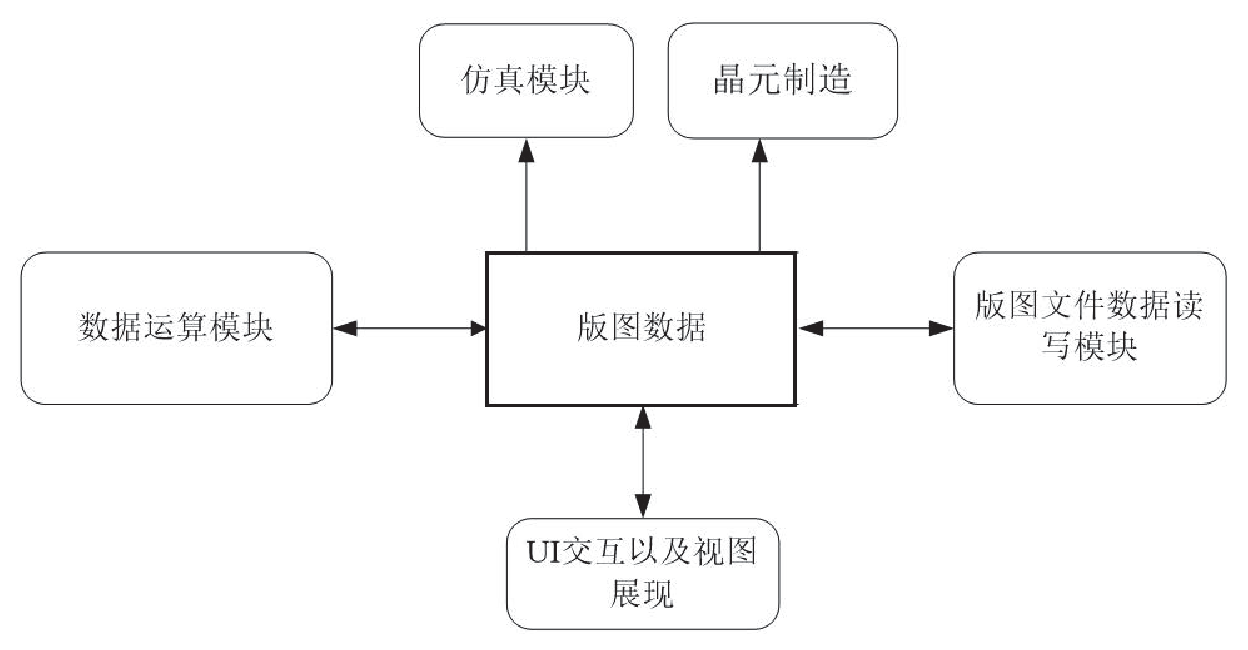
\includegraphics[width=6in]{./Layout/FigsArch/LayoutArchitect.eps}
	\caption{Optixera Software Architecture.}
	\label{FigLayoutArch}
\end{figure}

\subsection{目前存在的问题} \label{SectArchIssue} 
目前存在的问题:
\begin{enumerate}
	\item 并没有一个通用的版图数据结构,数据只是简单实用QGraphicsItem子对象来表示并保存,这样明显是没法实际操作的。以后的一些运算仿真就会比较麻烦甚至没法做。
	\item 对于版图中各种元素绘制,也是直接采用QGraphicsItem子对象来表示图元。这种方式的优点节省了代码量,很多细节不需要关心。缺点是资源耗费增大,有些特殊应用可能比较难以实现,例如也许修改会比较麻烦。我还要评估一下这样的效率和资源耗费。以及坐标转换后是否导致精度损失。
	\item 目前实现的操作好像都是针对单个图元,不能针对一组甚至全部数据。例如undo。
	\item 源代码目录结构不要随意变更
\end{enumerate}

%======================================================================
\section{基础数据结构模块} \label{SectArchData}
%======================================================================
基础数据结构模块如Figure (\ref{FigLayoutDataArch})所示。
\begin{figure}[htb!p] %h--here, t--top, b--bottom, p--page;
	\centering
	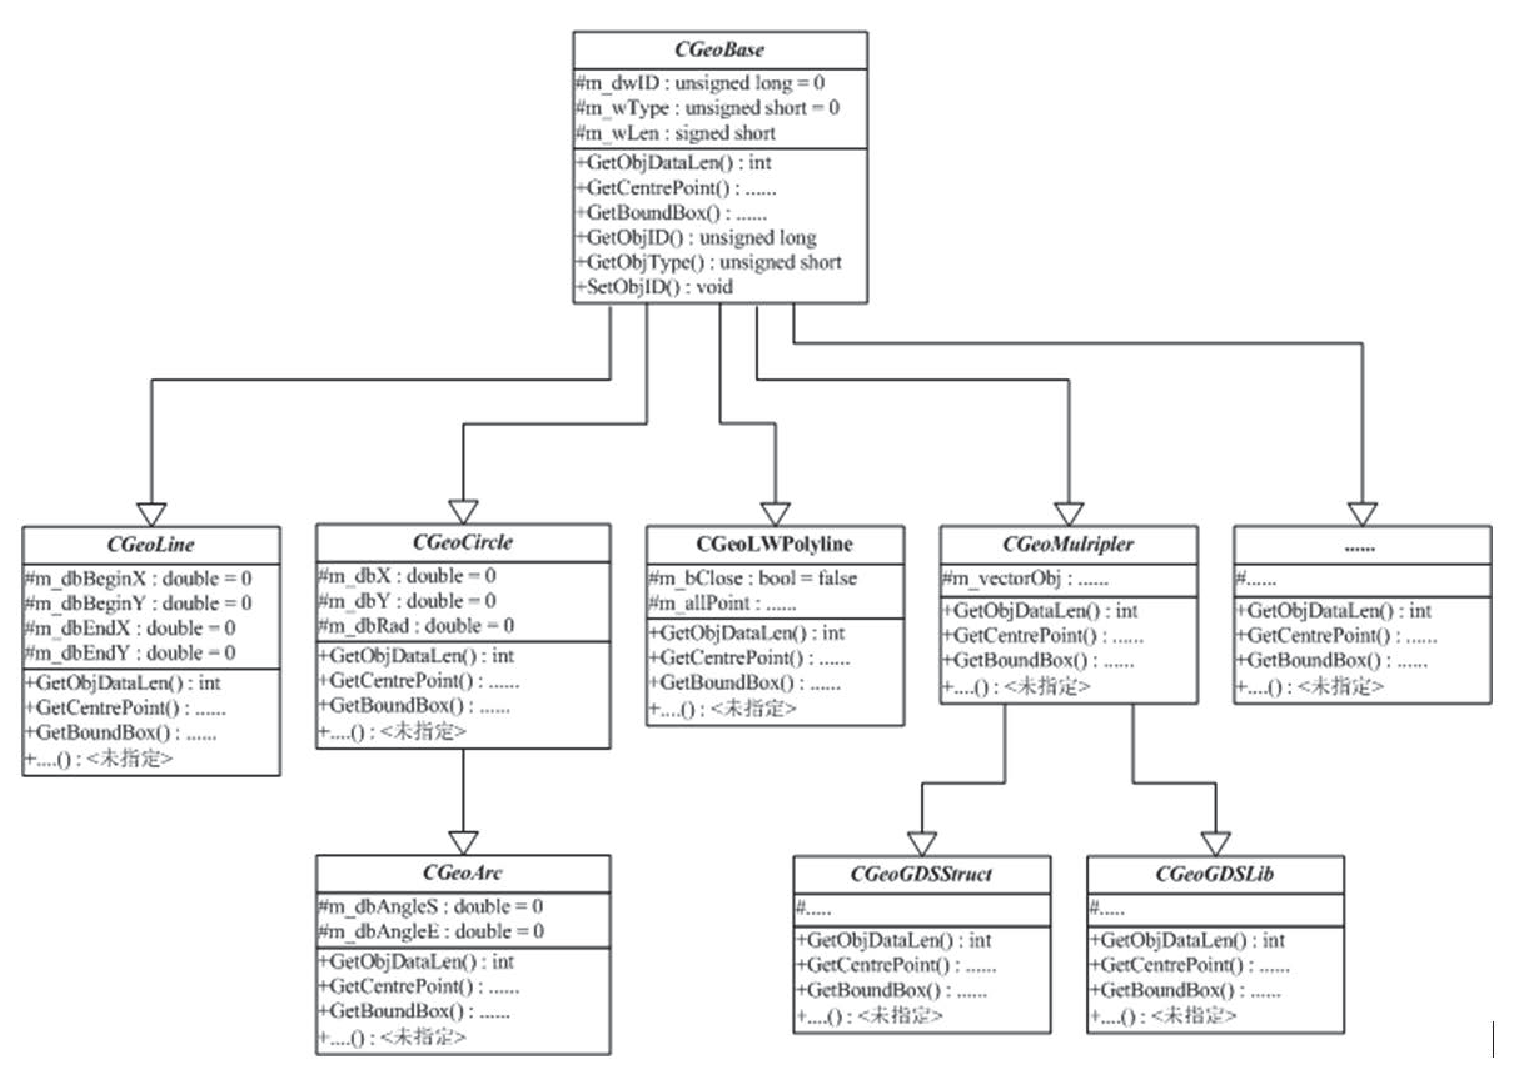
\includegraphics[width=6in]{./Layout/FigsArch/LayoutDataStructure.eps}
	\caption{Optimask Layout Data Architecture 版图数据类结构描述图样。}
	\label{FigLayoutDataArch}
\end{figure}

%======================================================================
\section{版图文件读写模块} \label{SectArchFileRW}
%======================================================================
\subsection{版图数据类结构描述图样} \label{SectArchFileStrc} 
版图文件数据读写模块的代码逻辑结构如Figure (\ref{FigLayoutDataArch})所示。
\begin{figure}[htb!p] %h--here, t--top, b--bottom, p--page;
	\centering
	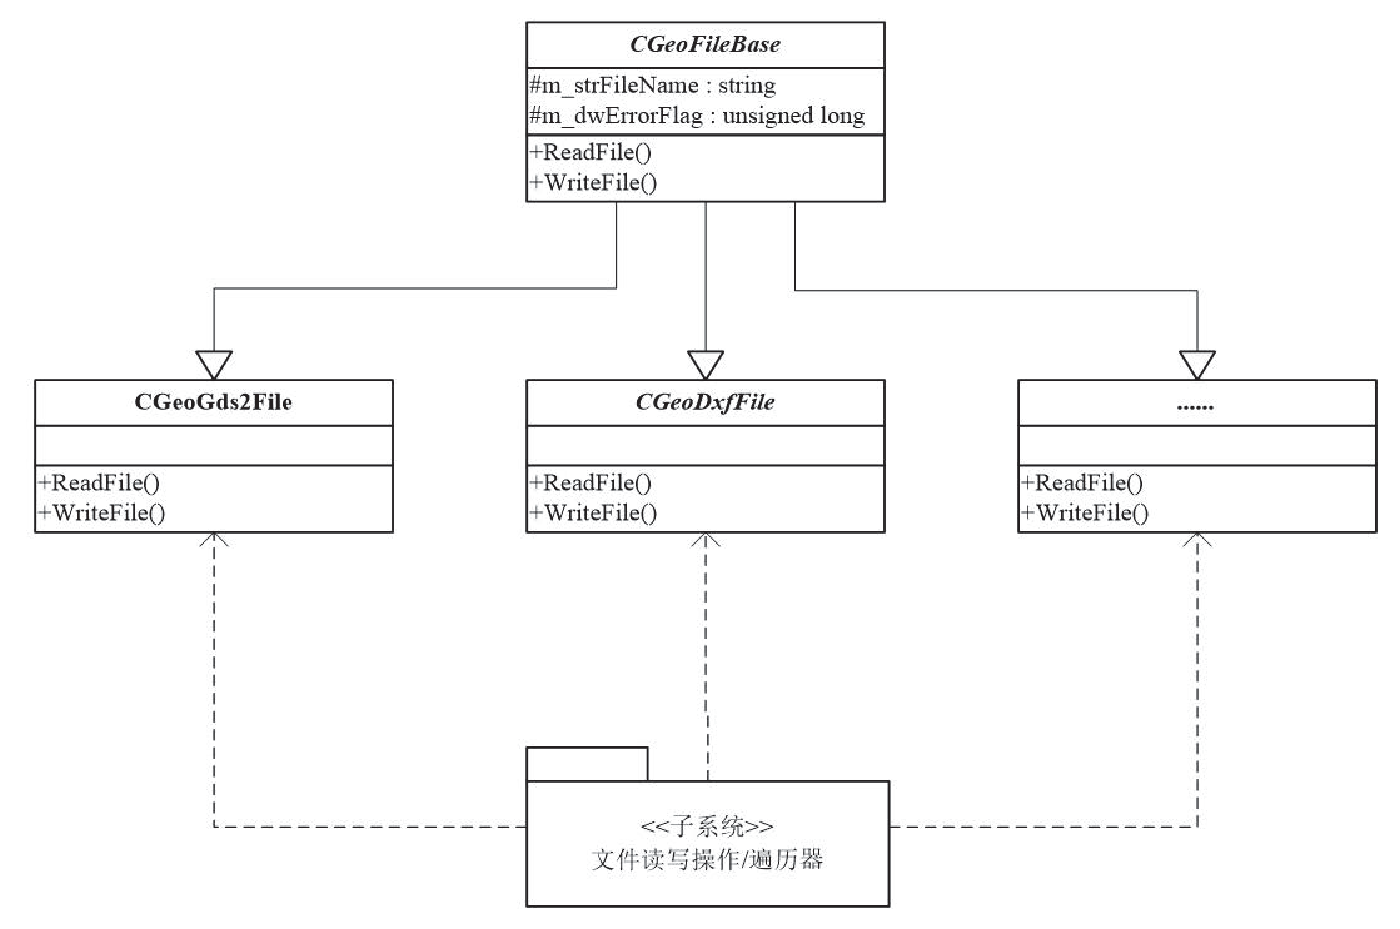
\includegraphics[width=6in]{./Layout/FigsArch/LayoutFileRWmodule.eps}
	\caption{Optimask Layout File Read/Write Module Architecture 版图文件读写模块。}
	\label{FigLayoutFileArch}
\end{figure}

\subsection{注意点描述} \label{SectArchFileNote} 
文件数据读取基类CGeoFileBase代码在GeoFile.h中,任何格式的文件实现代码必须派生与CGeoFileBase类,必须实现两个基本的虚函数ReadFile()和WriteFile(),前者是把文件数据解析成场景数据CGeoScene,后者把场景数据保存为指定格式的文件。除了两个基本的虚函数,以后可能还要添加其他的基础函数,例如GetErrorInf(),用于读取或者写入文件失败后,获取更详细的错误信息。

一个派生类至少要实现一种文件格式的读取,当然也可以同时实现几种格式的读取。对于任何格式文件的文件解析,必须实现读取函数ReadFile()用于读取指定格式的文件数据。但是根据实际情况是否特别需要,可以有选择的实现WriteFile()函数。

任何派生类都必须有缺省构造函数,因为文件读写操作/遍历器根据不同格式生成对应派生类对象时调用的是缺省构造函数。

文件读写操作/遍历器子程序包括一系列的宏定义和两个读写函数,具体列举如下:
\begin{enumerate}
	\item 全局函数$ReadDataFromFile()$和$WriteDataToFile()$
	\item 宏定义$DECLARE\_FILEFORMAT(class\_name)$声明文件格式操作链接
	\item $BEGIN_REGISTRATION(class\_name)$和$END_REGISTRATION(class\_name)$宏定义用于实现文件格式操作链接
	\item $REGISTRATION\_EXT(class\_name,ext\_name)$宏定义用于添加该类支持哪些格式解析。
\end{enumerate}

有了这些宏定义后,以后扩展或者删除其他格式解析的类代码时,只需要针对具体的格式解析类做相关的操作,其他的代码都不需要修改。因为有了这些宏的定义,$ReadDataFromFile()$和$WriteDataToFile()$函数就跟自动遍历所支持的格式类并且生成相应的类对象然后操作这些对象进行读取或者写入操作。

如$ReadDataFromFile("aaa.dxf")$。则内部根类型名找到$CGeoDXFFile$类并生成$CGeoDXFFile$对象,然偶把文件名参数以及其他的必要参数传递进入后调用$CGeoDXFFile::ReadFile()$把文件数据读取到$CGeoScene$对象中。$WriteFile()$也类似。

这些宏定义是自动遍历的基础,如果没有这些宏定义,每次增加新的格式解析类或者删除已有的格式解析类, $ReadDataFromFile()$和$WriteDataToFile()$函数代码都要相应的修改。

宏定义的使用方法:
\begin{enumerate}
	\item $DECLARE_FILEFORMAT(class\_name)$宏定义添加在每个派生的具体格式文件解析类的定义末尾,其中$class\_name$为派生类的类名。如下:
	\begin{lstlisting}[language=C]
		class CGeoDXFFile : public CGeoFileBase
		{
		……  //其他代码
		DECLARE_FILEFORMAT(CGeoDXFFile)
		};
	\end{lstlisting}
	
	\item 
	在派生类的实现文件文件中的开头添加剩下的三个宏定义,
	$BEGIN\_REGISTRATION$,$REGISTRATION\_EXT$,$END\_REGISTRATION$。
	示例如下:
	\begin{lstlisting}[language=C]
		include "GeoDxfFile.h"
		… //其他包含文件以及其他数据
		BEGIN_REGISTRATION(CGeoDXFFile)
		REGISTRATION_EXT(CGeoDXFFile, TEXT("DXF"))
		REGISTRATION_EXT(CGeoDXFFile, TEXT("DWG"))
		END_REGISTRATION(CGeoDXFFile)
	\end{lstlisting}
	
	\item
	支持一种格式,就使用$REGISTRATION_EXT(class\_name,ext\_name)$ 添加。如果支持多种格式,则每种格式都调用一次,如上的示例代码同时支持$dxf$和$dwg$格式。$class\_name$表示派生类名,$ext_name$表示支持的格式名称。
\end{enumerate}
注意:$REGISTRATION\_EXT$必须在$BEGIN\_REGISTRATION$和$END\_REGISTRATION$宏定义的中间。

%======================================================================
\section{功能清单Function CheckList} \label{SectArchFuncList}
%======================================================================
\begin{enumerate}
	\item 完善版图基础图元基础数据结构和文件数据结构定义
	\item 在Qt中实现版图基本图元自画。基本图元包括点,线,圆,圆弧,椭圆,多义线(区域)
	\item 实现基本图元的绘制数据从基础数据结构获取
	\item 在Qt中实现基本图元的选取,要注意多个图元有重叠的情况,这种情况要选取最上面的一个
	\item 实现对自画的基本图元移动缩放等处理
	\item 实现把GDS文件读入版图基础数据结构
	\item 实现版图基础数据结构数据写入到把GDS文件
	\item 实现dxf文件基本的数图元据读取
	\item 替换原先的Qt预定义图元和文档对象中的数据结构
	\item 命令行中画图调用的函数与主绘图中调用函数统一
\end{enumerate}

%======================================================================
\section{功能描述Function Description} \label{SectArchFuncDesc}
%======================================================================
根据以上的功能清单,把各个功能的开发以及一些功能实现的方案描述和工作安排。

\subsection{完善版图基础图元数据结构} \label{SectArchTaskDataStrc} 
完善版图基础图元数据结构和文件数据结构定义以及相关的数据读取功能,要求达到的最终目的如下:
\begin{enumerate}
	\item 基础数据结构完全兼容GDS2文件格式数据、大部分兼容DXF文件格式。
	\item 完善现有的GDS2文件数据读取,使之能够完整的解析出GDS2文件数据。
	\item 把读取的GDS2文件的数据转化为场景数据结构
	\item 实现把版图场景数据写入到GDS2文件中
	\item 实现把基本DXF文件数据读取到版图场景数据中
	\item 该功能估计工作量2~3周。
\end{enumerate}

\subsection{实现基本图元的绘制数据} \label{SectArchTaskDataDraw} 
实现基本图元的绘制数据从最新的版图场景数据结构中获取该功能要求绘图的数据源必须从最新定义的版图场景数据结构里面获取。以画线为例:
\begin{lstlisting}[language=C]
CGeoPt ptStart,ptEnd;
CGeoLine* temp = static_cast<CGeoLine*>(pObj);
ptStart = temp->GetFirstPt();
ptEnd = temp->GetSecondPt();
QgraphicsLineItem *item = new QgraphicsLineItem 
    (ptStart.dx, ptStart.dy, ptEnd.dx, ptEnd.dy);
item->setFlags(QGraphicsItem::ItemIsSelectable | QGraphicsItem::ItemIsMovable);
item->setPen(pen);
addItem(item);
item->setPos(0,0);
\end{lstlisting}
这个功能中的自定义在下一个功能描述中也会涉及到。这个功能由于这一步只是做一些数据源的替换实现。为了简化,可以把现有的绘制场景代码复制过来修改其中传入的参数,实现可以参考第四步。当然也可以与第四步的场景渲染结构合并一块进行,如果不合并,这个工作量比较少,估计2~3天。

\subsection{在Qt中实现版图基本图元自画} \label{SectArchTaskQtDraw} 
这个功能要求把以前在Qt中通过QGraphicsItem类的子类对象画基本图元全部改成自画,例如上一步描述的就是通过QgraphicsLineItem实现画线,经过这一步后不再使用QGraphicsItem类的子类对象实现,也不需要通过addItem(item)之类的代码把该图元添加到场景中。可以减少实现数据渲染依赖具体UI对象。

还是以上面的画线为例,修改后画图的示例代码如下:
\begin{lstlisting}[language=C]
CGeoPt ptStart,ptEnd;
CGeoLine* temp = static_cast<CGeoLine*>(pObj);
ptStart = temp->GetFirstPt();
ptEnd = temp->GetSecondPt();
QpointF tmpStart(ptStart.dx, ptStart.dy);
QpointF tmpEnd(ptEnd.dx, ptEnd.dy)

QPainter painter(this->viewport());
QPen pen(Qt::black);    
painter.setPen(pen);
painter.setBrush(Qt::black);
painter.drawLine(tmpStart, tmpEnd);
\end{lstlisting}
注意:以上代码只是一个简单的演示代码。对于实际上的场景画图,画图时不要直接画到显存上,而是要先画到位图上,然后把位图复制给显存。这些绘制可以在paintEvent事件里面画图,也可以独立,根据实际情况来。

为了方便场景数据的绘制,定义了一个场景渲染接口类CSceneRender用于封装与UI绘制无关的绘制操作,在其子类里面实现与具体的UI接口关联绘制,接口定义在SceneRender.h文件中。该接口类定义了一些基础图元绘制函数接口,由子类实现绘制。

接口定义如下,以后也许会增加或者修改接口定义
\begin{lstlisting}[language=C]
virtual void DrawScene();
virtual void DrawPrimitive(CGeoLine* pData)=0;
virtual void DrawPrimitive(CGeoCircle* pData)=0;
virtual void DrawPrimitive(CGeoArc* pData)=0;
virtual void DrawPrimitive(CGeoLWPolyline* pData)=0;
virtual void DrawPrimitive(CGeoEllipse* pData)=0;
virtual void DrawPrimitive(CGeoText* pData)=0;
virtual void DrawPrimitive(CGeoMulripler* pData)=0;
\end{lstlisting}

在上面的定义中,DrawScene()函数接口用于绘制整个场景,它的实现是遍历整个场景所有图层中的所有图元(如果某个图元有子图元,则迭代遍历,直达基本图元的叶节点),然后分别画出基本图元。
DrawPrimitive()函数分别对应着不同的基本图元实现不同的绘制方法。例如$DrawPrimitive(CGeoLine* pData)$函数的实现绘制直线,可能是如下的情况:
\begin{lstlisting}[language=C]
DrawPrimitive(CGeoLine* pData)
{
	CGeoPt ptStart,ptEnd;
	ptStart = pData ->GetFirstPt();
	ptEnd = pData ->GetSecondPt();
	如果没有实现自定义绘制,则应该是如下的代码
	QgraphicsLineItem *item = new QgraphicsLineItem
	    (ptStart.dx, ptStart.dy, ptEnd.dx, ptEnd.dy);
	item->setFlags(QGraphicsItem::ItemIsSelectable 
	    | QGraphicsItem::ItemIsMovable);
	item->setPen(pen);
	addItem(item);
	//如果采用的自定义绘图,则是类似如下的代码
	//(仅仅是示例用来表明方案,实现上根据实际情况可能采用效率更高的绘制)
	QpointF tmpStart(ptStart.dx, ptStart.dy);
	QpointF tmpEnd(ptEnd.dx, ptEnd.dy)
	QPainter painter(this->viewport());
	QPen pen(Qt::black);    
	painter.setPen(pen);
	painter.setBrush(Qt::black);
	painter.drawLine(tmpStart, tmpEnd);
}
\end{lstlisting}

场景接口类必须与具体的UI操作结合来实现绘图,绘图操作与场景渲染接口类CsceneRender结合的代码如下:
以Qt的视图绘制类为例:

\begin{lstlisting}[language=C]
class CView:public QgraphicsView, public CSceneRender
{
	Q_OBJECT
	
	….
	virtual void DrawScene();
	virtual void DrawPrimitive(CGeoLine* pData);
	virtual void DrawPrimitive(CGeoCircle* pData);
	virtual void DrawPrimitive(CGeoArc* pData);
	virtual void DrawPrimitive(CGeoLWPolyline* pData);
	virtual void DrawPrimitive(CGeoEllipse* pData);
	virtual void DrawPrimitive(CGeoText* pData);
	virtual void DrawPrimitive(CGeoMulripler* pData);
}
\end{lstlisting}

该场景类也定义了一些基本的场景图元添加删除更新操作,方便命令行功能模块调用这些接口函数实现场景相关的操作诸如添加直线等。如
AddLine()

DelObject()

命令行功能如果接收到输入添加直线的命令,解析后直接调用AddLine(),该函数自动把新增的直线添加到当前场景数据中,如果同时需要把添加的直线在视图上显示出来,则调用DrawPrimitive()函数即可。

场景渲染结构示意图如下:

\subsection{在Qt中实现自画基本图元的选取} \label{SectArchTaskQtPick} 
选取基本图元的功能是基于自定义画图,如果采取Qt的预定义绘图,则内置了选取移动等功能,选取功能不需要再次实现。

进行图元选取之前,先必须建立基于坐标位置的图元索引,建立图元索引的方案描述如下:
\begin{enumerate}
	\item 把整个场景分成n*m个栅格区域,每个栅格的编号都是根据实际坐标范围来映射,每个编号本身的含义就对应着一定的栅格区域范围。每个栅格的大小固定的。
	\item 计算栅格编号的方法:先计算出图形区域的最小坐标点$(Xmin,Ymin)$和最大坐标点$(Xmax,Ymax)$。最小坐标点向下取整,最大坐标点向上取整。为了冗余,也可以在最小坐标点再向下偏移几个单位,最大坐标点再向上偏移几个单位。然后计算出栅格的区域范围,其中宽度数据$width=(Xmax- Xmin)/n$,高度数据为$height=(Ymax- Ymin)/m$。计算出来的宽度和高度向上取整。对于任意坐标$(X,Y)$,则$X$方向的编号为$NOx =  (X- Xmin)/width$, $Y$方向的编号为$NOy =  (Y- Ymin)/ height$。两者编号都取整。实际编号就是两者编号的组合,如$NO = (NOx<<16)+ NOy$。(设定编号为32为无符号整形)。
	\item 如果图元位于栅格里面、与栅格相交、包含栅格。则这个图元就属于这个栅格。因此一个图元可能对应着多个栅格。建立一个编号与图元的多重映射,关键字为栅格编号,值为图元列表。
	\item 当图元发生平移或者选择时,需要更新该图元所在的栅格信息。
\end{enumerate}

选取的功能描述如下;
\begin{enumerate}
	\item 把选取的屏幕坐标转化为图形坐标
	\item 根据图形坐标计算该坐标所在的栅格ID
	\item 根据栅格ID找出位于该栅格的所有图元,然后继续下一步找出满足条件的图元。
	\item 把这个栅格内的所有图元的区域与选取的坐标点进行比较,如果坐标点位于区域内或者区域边界,则满足要求。如果有多个图元满足要求,则选取的原则为:就小不就大,当前层优先。意思如果多个图元都包含选取点时,则选取区域最小的那个,如果区域相同的有多个,则选取当前层的那个。另外如果当前层也有区域相同的多个(正常情况下这应该是错误,因为这是重复图元)则选列表中的第一个。
	\item 选定了基本图元,把图元的边界突出显示
\end{enumerate}

\subsection{对自画图元的平移旋转等基本操作} \label{SectArchTaskDrawAltr} 
平移旋转操作本身不是难事,现在主要说明在鼠标操作的情况:
\begin{enumerate}
	\item 选定需要操作的图元
	\item 捕获鼠标的点击与移动事件,计算出图元要平移或者旋转的屏幕距离
	\item 根据平移或者旋转操作把计算出来的屏幕距离转换成实际的平移距离或者选择的角位移
	\item 调用平移或者旋转函数
	\item 要求刷新显示
\end{enumerate}
如果是命令行,则只有后面的4,5两步。
目前需要把针对图元旋转平移的功能封装起来。

\subsection{彻底替换以前的采用Qt预定义图元操作以及文档中的场景数据} \label{SectArchTaskReplaceQt} 
彻底替换以前的采用Qt预定义图元操作以及文档中的场景数据。


%%\pagestyle{empty}
%%\cleardoublepage
%%to generates one blank page for the next chapter to be on an odd page

%% Main UI of Optimask Layout Software
%% Created: 2017-05-15; Updated: 2017-07-15;
%% by Henghua DENG, hdeng@optixera.com

\resetdatestamp %Date Stamp--Only use when custom package datestamp.sty is used.

%\part{Optimask Layout Design} \label{PartMaskDesign}
%本部分介绍Optimask版图设计软件基本框架,具体功能实现,主要界面,命令行及编程输入等等。

\chapter{Optimask基本界面} \label{ChMaskMainUI}
%======================================================================
%Heading Settings:
\markboth{Chapter~\thechapter.~Design~Architecture}{} %\leftmark calls #1 parameter
%\markright{ } % new right header. Only used for two-side documents.

\pagestyle{fancy}
\fancyhead[RO,RE]{}
\fancyhead[LE]{\MakeUppercase{\leftmark}}
\fancyhead[LO]{\MakeUppercase{\rightmark}}
\fancyfoot[C]{\thepage}
%%\fancyfoot[L]{\today}

目前我们的基本框架已经定型如下。
各区域缺省设置如上图。用户可在设置界面关闭或者取消指定区域,且可自由移动、放大和缩小区域。
具体到每个子区:

%======================================================================
\section{菜单栏(Menu)} \label{SectMaskMenus}
%======================================================================
% \OptiXera\Develop\optixera\Docs\软件开发代码规范.txt Optixera版图软件开发进阶.docx 

菜单栏包括通常的文件输入输出,程序设置,版图绘制,浏览编辑,程序调试,辅助工具,视窗选择,使用帮助等类别功能。

\subsection{文件(File)} \label{SectMaskMenuFile} 
程序的第一步操作是文件操作。
试验创建、打开、关闭文件。
试验导入导出“GDSII”文件。实例GDSII文档在
\begin{verbatim} \optixera\optimask\src\File\GDSII_Test_File \end{verbatim} 目录和
\begin{verbatim} \klayout-0.24.8\testdata\gds \end{verbatim} 目录。
试验导入导出“OASIS”文件。如下图所示。实例GDSII文档在
\begin{verbatim} \klayout-0.24.8\testdata\oasis \end{verbatim} 目录。OASIS文档和GDSII文档可以互相转换。
\subsubsection{File --> Import GDSII }
\begin{enumerate}
	\item 测试单个构元,单层。单个构元有多重部件。
	\item 测试单个构元,但是多层。
	\item 测试多个构元,而且多层。
\end{enumerate}

\subsection{编辑(Edit)} \label{SectMaskMenuEdit} 
\subsection{视图(View)} \label{SectMaskMenuView} 
\subsection{绘制(Draw)} \label{SectMaskMenuDraw} 

%i.	Polygon, Circle, Wire(用户可简单通过界面画图,鼠标或键盘。这是目前软件都可以做到的基本功能)
%ii.	Input by Matrix, or calculate polygon points.(这是目前所有版图软件无法独立做到的地方。) 
%iii.	扫描图形Scan Picture(这是目前版图软件比较难做到的地方)。也可扫描条形码,和二维码。算法存下的文件必须精确,且文件尺寸小。
%iv.	图形库(我们慢慢建立)。
%v.	字库。可引入任意字库(C:\Windows\Fonts)字体如上图例(而非限于仅有几个难看的字)。 

\subsection{变化(Alter)} \label{SectMaskMenuAlter} 
\subsection{构元(Cell)} \label{SectMaskMenuCell}
\subsection{构层(Layer)} \label{SectMaskMenuLayer}
\subsection{编程(Script, Code, Macro, Programming)} \label{SectMaskMenuCode} 
\subsection{配置(Config)} \label{SectMaskMenuCnfg} 
\subsection{工具(Tool)} \label{SectMaskMenuTool}
\subsection{窗口(Window)} \label{SectMaskMenuWndw} 
\subsection{帮助(Help)} \label{SectMaskMenuHelp}

%======================================================================
\section{工具条(Toolbar)} \label{SectMaskToolbar}
%======================================================================
工具条主要是对应菜单栏的所有功能。需要每个功能有对应的图标。每一个菜单栏所有的功能集中在同一个工具条上。

%======================================================================
\section{构层面板(Layer Panel)和构层配置(Layer Palette)} \label{SectMaskLayers}
%======================================================================
构层区和层设置区(Layers Palette)缺省随主界面,但是允许用户自由移动和关闭。(当层设置好后,有时用户需要大窗口进行绘图)

\subsection{构层面板(Layer Panel)} \label{SectMaskLayerPanel} 
构层面板(Layer Panel)主要是构层的列表。
其中表头分别为: Group, LAYER, Lock, Hide, Protect,Fill, GDSII Number(\#), GDSII Data Type (DT),Note。
表格数据为版图文件所真实包含的构层列表。对于每一构层,如果有对应表头的数据,那么就显示;如果没有表头对应的数据项,那么就显示为空即可。上图显示的表格数据只是一个虚例,真正的显示需要根据版图文件对应显示。
表格数据每一行对应一个构层。关于表头具体到单项:
\subsubsection{构层组群(Layer Group)或类别(Category)或排序(Order)}
构层组群(Layer Group)或类别(Category)或排序(Order)可以方便用户对多层组织,比如上图的群A有Chip和Mark两层。当然用户可以不组群,此时用户也可以通过这一栏设定特定的值来进行排序。
这里举个K-Layout参考示例 。对层群的操作需要传递到其从属的所有构层。
\subsubsection{构层名称(Layer Name)}
构层名称(Layer Name)记录构层的名称(必须有)。如果用户不给构层命名,那么程序可以自动设置构层名称为GDSII\#对应(读入GDSII文件一定有GDSII\#)。 比如Layer\#005(如果GDSII\#为5)。当然也有另外一种情况,有构层名称,但没有GDSII\#,这时表示该层不会输出到GDSII文件格式中去。
\subsubsection{锁定(Lock)}
是否锁定(LOCK=1加锁, UNLOCK=0解锁)。锁定某构层表示该构层不会被修改,即使用户修改了该层的物件,也不会允许被保存文件(此时可以弹出警告框提示)。锁定可以防止对指定层的误操作。所有可以修改的构层必须在解锁状态。
\subsubsection{隐藏(Hide)}
是否隐藏(HIDE=1=UNSHOW隐藏, UNHIDE=0=SHOW显示)。隐藏某构层时,在工作窗口上不会显示该层的任何图像。构层被隐藏时,也同时不可以被选中(即,同时处于PROTect状态)。
\subsubsection{保护(PROTect)}
是否保护(PROTect=1=Unselectable不可选中, UNPROT=0=Selectable可选中)。
\subsubsection{填充(Fill)}
是否填充(FILL=1实心, UNFILL=0空心)。选定是该构层的图形全部实心显示,否则空心显示。
\subsubsection{GDSII 层号Number (\#)}
导入导出时对应的GDSII构层号码。导入GDSII文件一定有GDSII\#。如果有构层名称,但没有GDSII\#,这时表示该层不会输出到GDSII文件格式中去。
\subsubsection{GDSII 数据类型(Data Type,DT)}
GDSII数据类型。
\subsubsection{注释(Note)}
对构层的注释(如果有必要)。可以为空白。

\subsection{构层配置(Layer Palette)} \label{SectMaskLayerPalette} 
构层配置(色板,格纹,动画,样式,能见度)基本套用KLayout 。其中(Optimask :KLayout)名字对应为: Fill Color = Color, Frame Color = Frame color, Pattern = Stipple; 其他不变。
构层色板(Layer Palette)包括下面子部分:
\subsubsection{构层格纹(Stipple, Pattern)}
\subsubsection{构层动画(Animation)}
\subsubsection{构层样式(Style)}
\subsubsection{构层能见度(Visibility)}

%======================================================================
\section{构元结构面板(Cell Structure Panel)} \label{SectMaskCellDock}
%======================================================================
CellDock构元结构面板(Cell Structure Tree Panel), 构元组织(Cell Hierarchy),模块树和组织结构区。显示各结构之间的从属关系。双击特定某个构元时,打开一个新工作窗口来显示该构元图形。

%======================================================================
\section{版图主视图区(Work Panel)} \label{SectMaskWorkDock}
%======================================================================
WorkDock版图主视图区 ---- 主要版图设计工作区。结构的绘图,调用,几何运算,显示等等。允许多重工作区域(Workspace, Work Panel)。

%======================================================================
\section{视图导航区域 (Navigator, Aerial View)} \label{SectMaskNaviDock}
%======================================================================
NaviDock视图导航区域 (Navigator, Aerial View) (导航区,鸟瞰区,第二视图区,辅助视图区)--- 显示当前结构在整个Wafer组装之后的位置等等。鼠标选中对应的位置时,主工作区可以显示该地方的详尽图;反之亦然。

%======================================================================
\section{编程区域(Command, Script, Macro, Code, Programming)} \label{SectMaskCodeDock}
%======================================================================
CodeDock编程区域(Command, Script, Macro, Code, Programming)---编程产生结构,以及结构组合宏命令(比如Assembling)上。

%======================================================================
\section{信息输出栏(Information, Status, Result, Output)} \label{SectMaskInfoDock}
%======================================================================
InfoDock信息输出栏(Information, Status, Result, Output) --- 显示程序运行时必要的显示信息,输出结果等等。显示当前结构的统计信息,比如多少层,多少多边型,多少精度等等。

%======================================================================
\section{提示报警栏(Hint, Error, Warning, Issue)} \label{SectMaskHintDock}
%======================================================================
HintDock提示报警栏(Hint, Error, Warning, Issue)报错和提示区---如果程序出错,提示如何纠正。

%%\pagestyle{empty}
%%\cleardoublepage
%%to generates one blank page for the next chapter to be on an odd page

%% Optimask Commands and Scripts
%% Created: 2017-05-15; Updated: 2017-07-15;
%% by Henghua DENG, hdeng@optixera.com

\resetdatestamp %Date Stamp--Only use when custom package datestamp.sty is used.

%\part{Optimask Layout Design} \label{PartMaskDesign}
%本部分介绍Optimask版图设计软件基本框架,具体功能实现,主要界面,命令行及编程输入等等。

\chapter{Optimask Commands and Scripts} \label{ChMaskCmdScript}
%======================================================================
%Heading Settings:
\markboth{Chapter~\thechapter.~Command~Script}{} %\leftmark calls #1 parameter
%\markright{ } % new right header. Only used for two-side documents.

\pagestyle{fancy}
\fancyhead[RO,RE]{}
\fancyhead[LE]{\MakeUppercase{\leftmark}}
\fancyhead[LO]{\MakeUppercase{\rightmark}}
\fancyfoot[C]{\thepage}
%%\fancyfoot[L]{\today}

命令(Command)和脚本(Script)是非常有用的功能。目前其他软件的命令和脚本功能,或者功能太弱,或者太复杂,或者太难使用。在Optimask软件下,我们将定义非常简单高效的命令和脚本。

%======================================================================
\section{命令和脚本的基本原则} \label{SectCmdRule}
%======================================================================
Optimask软件中,命令和脚本的基本原则是简单高效易使用,对于用户而言是非常浅显易记的语言(Plain Language)。命令、脚本或宏的输入是在CodeDock命令输入窗口(见Figure (\ref{FigCodeDock}))交互输入和执行的。

\begin{figure}[htb!p] %h--here, t--top, b--bottom, p--page;
	\centering
	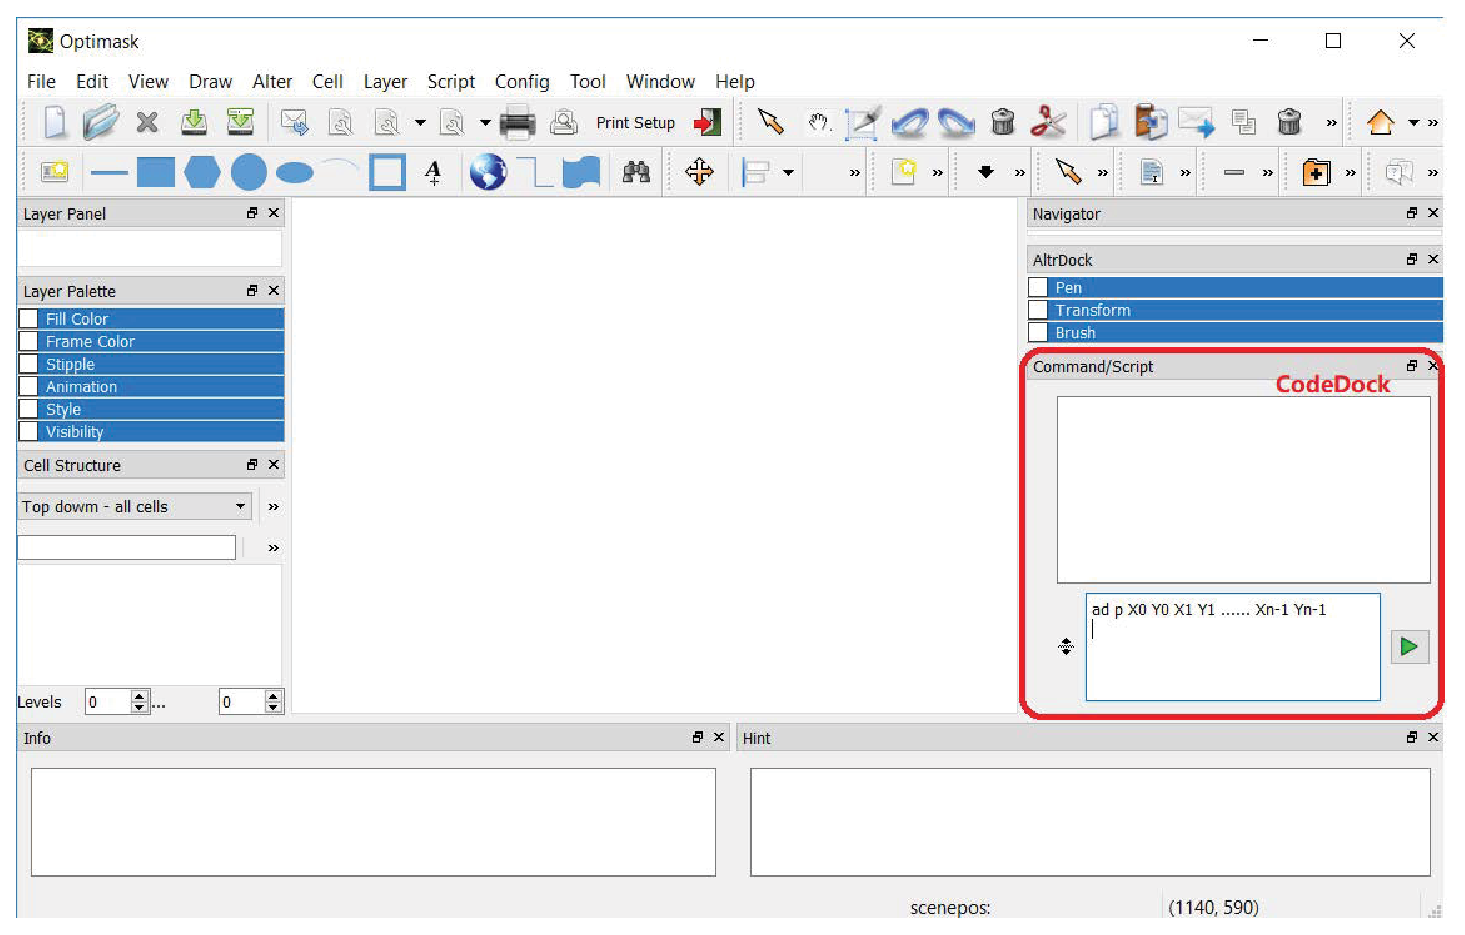
\includegraphics[width=4in]{./Layout/FigsCmd/CodeDock.eps}
	\caption{CodeDock for Command/Script/Macro input.}
	\label{FigCodeDock}
\end{figure}

\subsection{实时输入和文件运行} \label{SectCmdInput} 
允许实时输入,允许多行命令同时输入和执行,允许存储命令记录为文档,允许导入命令脚本文件直接执行。

文件存储为文本文件,便于用户阅读和修改。

命令可以通过命令输入窗口交互输入执行,也可以通过导入命令文件后执行。界面窗口有历史命令导出为文件的按钮,也有导入命令文件的按钮。导入命令文件之后可以点击执行(RUN)按钮。

此外还有一个选择是可以通过在命令输入窗口输入@符号加上文件名(可以不指定文件后缀),即文件运行使用\emph{@文件名})。比如如果命令文件名为AWG.cmd,那么在命令输入栏输入
\begin{verbatim} @AWG \end{verbatim} 
就等同于打开(OPEN)此文件后再执行(RUN)。

注意,命令文件的文本里面同样可以允许\emph{@文件名}的使用,即允许文件的嵌套调用。这样就大大扩展了命令和脚本文件的使用灵活性和功能性。

\subsection{命令注释} \label{SectCmdComment} 
文件中,注释允许多重注释符号,以扩展代码的灵活性和兼容性。允许的注释符号包括:
%%标准C/C++注释符(//, /* */)亦即Java注释符(//, /* */), Matlab注释符(\%)亦即\LaTeX注释符(\%), Python注释符(\#), DOS注释符(!)。
\begin{itemize}
	\item 标准C/C++注释符(//, /* */),亦即Java注释符,及L-Edit的T-Cell注释符
	\item Matlab注释符(\%),亦即LaTeX注释符(\%)
	\item Python注释符(\#)
	\item DOS注释符(!),亦即IC Editor注释符(!)
\end{itemize}

这些注释符号可以随意出现的命令和文件的任何位置。所有这些注释符号以及直到行末的文本在编译时都将被忽略。

\subsection{命令解析} \label{SectCmdIntrp} 
命令解析主要在后台自动进行。好的解析可以允许用户有适当的自由度,在适当的时候允许用户调整命令格式,以简化用户的计算和简化输入。
\subsubsection{模糊识别和自动输入} \label{SectCmdFuzy} 
命令和脚本解析允许模糊识别功能,且不分大小写。
比如添加多边形,
Add Polygon at (X0, Y0),  (X1, Y1), ......, (Xn-1, Yn-1);
等同于
ad p X0 Y0 X1 Y1 ...... Xn-1 Yn-1
如果以p开头的命令只有polygon。
假设以p开头的命令只有polygon和polyline,那么必须用户输入到polyg才可以区别。以此类推。
不区别大小写。
对于坐标组,是否有括符 (), [], \{\}都没关系,是否有逗号或分号分隔都没关系。

已添加矩形为例,命令如下:
Add Rectangle
Add Rect
Add Box
坐标只需要
X0 Y0 X1 Y1 
即左下角和右上角的两个定点坐标。
如果add已经可以用ad足够区分,如果没有R或B开头的关键词跟在Add 后面,那么
ad b
也可以工作。

\subsubsection{基本格式和变形格式} \label{SectCmdForms} 
对于每个命令,缺省有一个基本格式,同时可能有存在的变形格式。

对于任何一个基本图形,需要确定一个基本格式,比如
add box X0 Y0 X1 Y1 (W)
为添加矩形的基本命令格式。它确定一个(X0,Y0),(X0,Y1),(X1,Y1),(X0,Y1)的矩形,其各边均与(X,Y)坐标平行。

此基本格式不需要输入额外的变量名字,即后面的参数全为数字即可自动解析。但是如果希望以其他变形格式输入时,就需要输入变量名字和数值。比如

add box X0 Y0 X1 Y1 (W) rotateangle=90deg (rotatecenter=(Ox,Oy))

就会将此box对应rotatecenter旋转rotateangle。
其中rotatecenter缺省为box的中心点,如果用户指定rotatecenter=(Ox,Oy)那么就沿此(Ox,Oy)进行旋转。

同一个命令可以有多个变形格式,比如

add box Origin=(Ox,Oy) Width=10 Height=20 (W)

就会建立一个以(Ox,Oy)为中心,长度为10,高度为20的矩形,线宽W缺省为0。
或者

add box Base=(X,Y) Width=10 Height=20 (W)

就会建立一个以(X,Y)为左下角,长度为10,高度为20的矩形,线宽W缺省为0。

变形格式可以在后台全部自动转换为基本格式进行处理。如果是图形窗口(GUI)读取的命令,基本上可以转换为基本格式自动存储和计算。

\subsubsection{复合格式} \label{SectCmdCmb} 
同时可以允许有复合格式,即两个命令的混合。

比如命令1:
add box X0 Y0 X1 Y1 (W) 为添加矩形,

而命令2:
rotate angle center
将图形对应旋转中心center 坐标(Ox,Oy),旋转angle角度的操作。
那么
add box X0 Y0 X1 Y1 (W) rotate angle center
即为将此矩形产生和同时进行旋转操作。

其实该复合格式等同于同时执行两条命令:

add box X0 Y0 X1 Y1 (W)

rotate angle center

操作的目标缺省定义为最近绘制的那个图形。

\subsection{参数惯例} \label{SectCmdConvention} 
建议写程序代码时参数命名始终遵循下面这些惯例。但是对于用户是透明的。
\begin{enumerate}
	\item 大写(X,Y)为绝对坐标值,小写(x,y)为相对坐标值。换算关系为(X,Y)=(Ox,Oy)+(x,y),其中(Ox,Oy)为相对坐标系的原点在绝对坐标系中的坐标位置。
	\item angle为角度(degree),ang为弧度(radian)。二者换算关系为$ang=\dfrac{angle*\pi}{180}$和$angle=\dfrac{ang*180}{\pi}$。如果定义$deg=\dfrac{\pi}{180}$和$rad=\dfrac{180}{\pi}$,那么简单地通过2*deg就将角度$2^{\circ}$转换成弧度$\dfrac{\pi}{90}$,而$\dfrac{\pi}{4}*rad$就将弧度$\dfrac{\pi}{4}$转换成角度$45^{\circ}$。
	\item res为角弧精度(即对于弧线,变为多边形时,隔几度一个点),缺省单位为弧度(radian),缺省值为2*deg。
	\item (Ox,Oy)一般表示坐标系原点或圆心的绝对坐标位置。
	\item R为Radius(半径),等于直径的一半。
	\item W为线宽,缺省为0,表示没有线宽。(比如Add Circle如果W=0,那么产生实心圆形;否则就产生有线宽的圆环,内径的半径为R-0.5W,外径的半径为R+0.5W。)
\end{enumerate}

%======================================================================
\section{命令总览} \label{SectCmdCtgr} %Command Category
%======================================================================
命令总览可参考思维导图(XMind)文件
\begin{verbatim} \optixera\Docs\Optimask_File_Format.xmind \end{verbatim}。
命令总览见Figure (\ref{FigCmdOverview})所示,包含几个基本类别,如编辑、绘制、构元、视图、特性、变化等。下面依次介绍各类命令下的基本命令。
\begin{figure}[htb!p] %h--here, t--top, b--bottom, p--page;
	\centering
	\subfigure[Command Category(命令类别)] {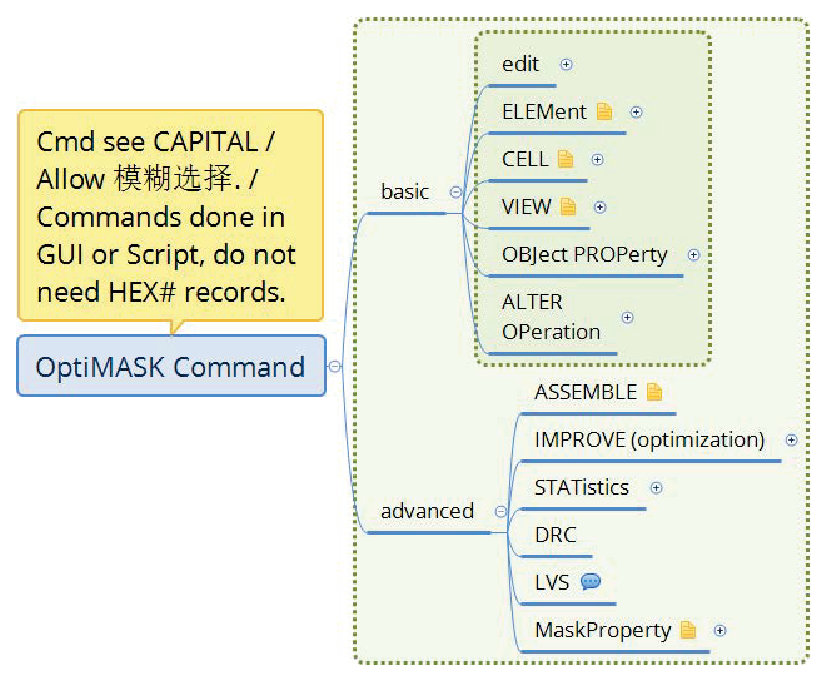
\includegraphics[width=3in]{./Layout/FigsCmd/CmdCategory.eps}
		\label{FigCmdCtgry}}
	\hfill
	\subfigure[Command Minimum Set(命令最小子集)] {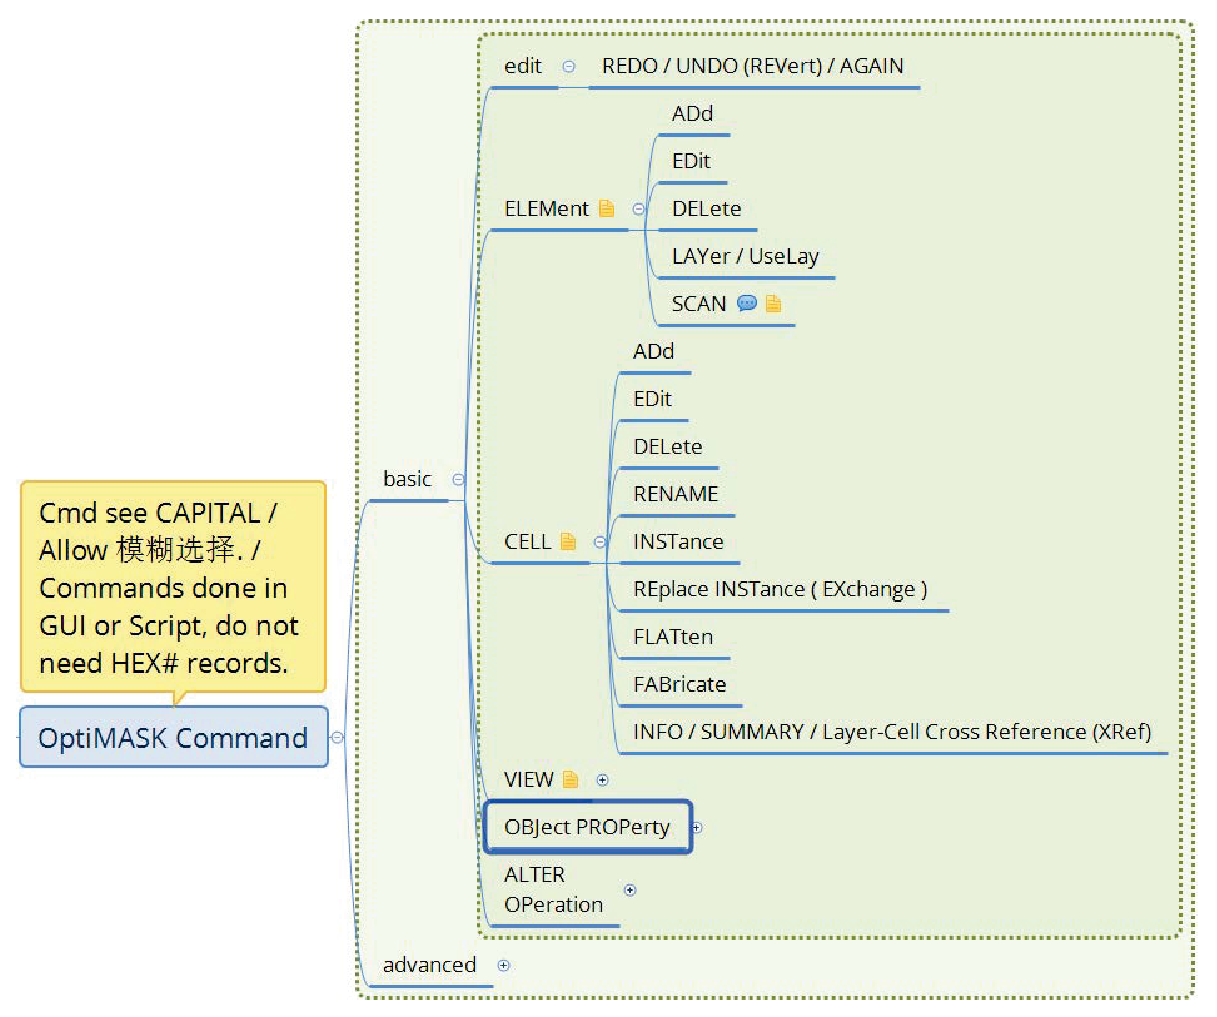
\includegraphics[width=3in]{./Layout/FigsCmd/CmdMinSet.eps}
		\label{FigCmdMinSet}}
	\caption{Overview of Commands 命令总览。}
	\label{FigCmdOverview}
\end{figure}

\subsection{编辑(Edit)} \label{SectCmdEdit}
操作REDO(AGAIN) / UNDO (REVert),主要针对最后一个命令行。这些对应界面的撤销和重复的动作。

Edit(编辑)的具体操作可以针对某个基本图元(Element),也可以针对某个复合构元(Cell),相应的Edit(编辑)将在对应的命令类别下面单独详细阐述。

\subsection{基本图形(Element)} \label{SectCmdDraw}
绘制基本图形(Draw Element)的操作命令见Figure \ref{FigCmdElem}。
\begin{figure}[htb!p] %h--here, t--top, b--bottom, p--page;
	\centering
	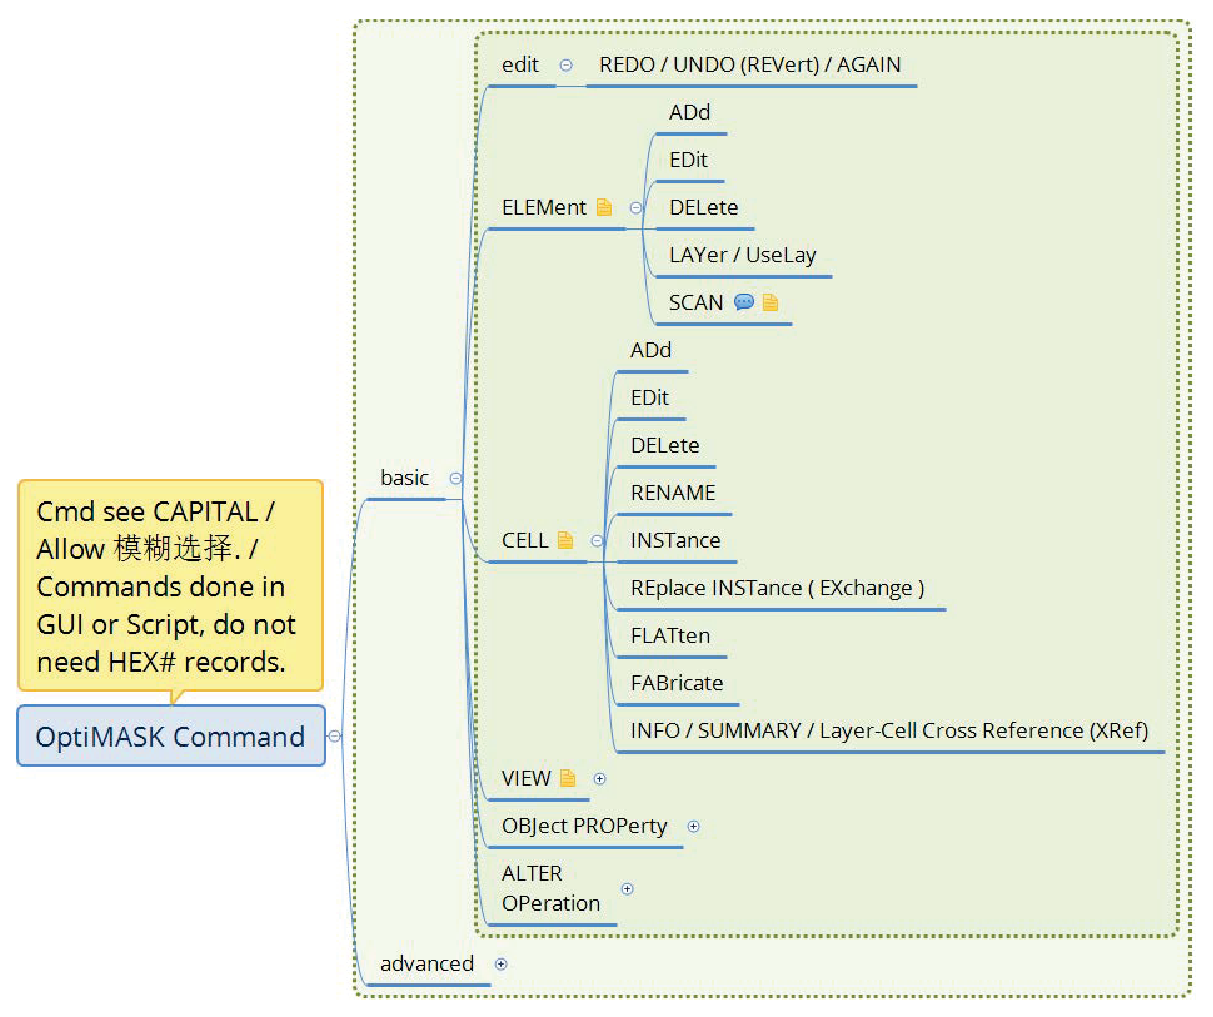
\includegraphics[width=4in]{./Layout/FigsCmd/CmdBasicElement.eps}
	\caption{Commands to Create Basic Elements 绘制基本图形命令。}
	\label{FigCmdElem}
\end{figure}
可以有Add(添加)(Draw),Edit(编辑),Delete(删除),Layer(构层)(即UseLayer,使用层号),以及高级功能Scan(扫描)。

\subsubsection{添加图元(Add)} \label{SectCmdAdd}
添加图元(Add/Draw Element)可以使用Add(添加)命令。添加的常用基本图形的基本格式示例如下
\begin{itemize}
	\item add box X0 Y0 X1 Y1 (W)
	\item add polygon X0 Y0 X1 Y1 ...... Xn-1 Yn-1 (W)
	\item add circle Ox Oy R (res) (W)
	\item add arc Ox Oy R ang1 ang2 (res) (W) 
	\item add Figure (\ref{FigExtRefElem})下的更复杂图元。
\end{itemize}
其中括弧框中的变量(比如(W))为可选项;若不存在则使用缺省值(比如(W=0))。非括弧框中的变量为必须提供的变量参数。

\begin{figure}[htb!p] %h--here, t--top, b--bottom, p--page;
	\centering
	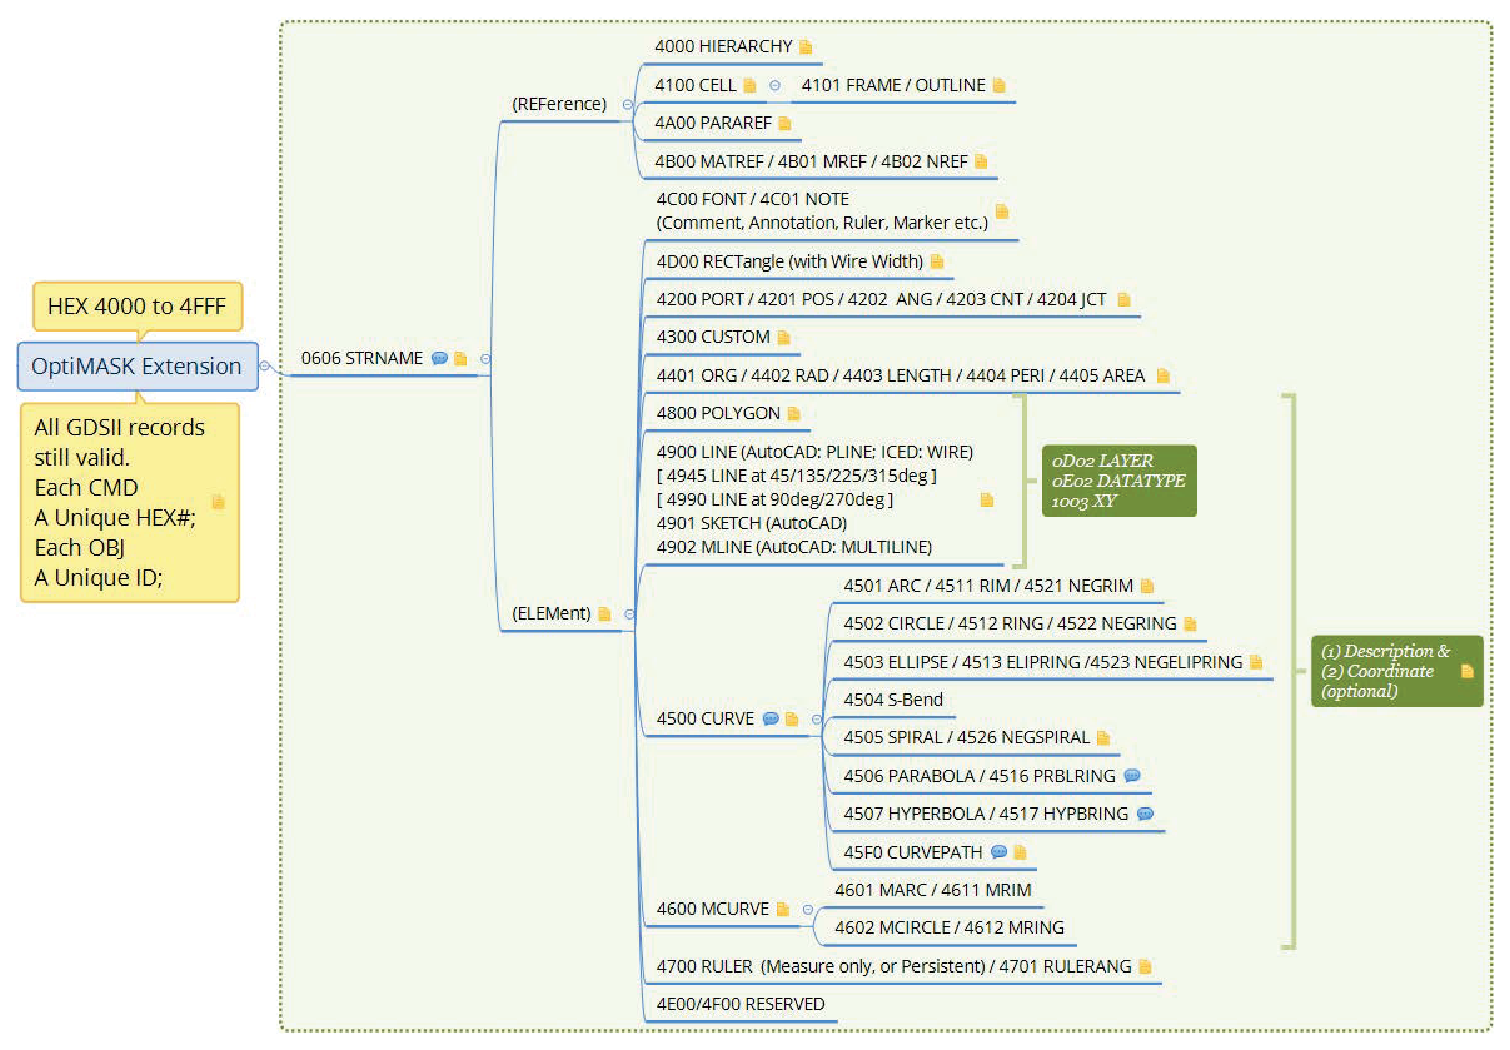
\includegraphics[width=4in]{./Layout/FigsCmd/Optimask_Ext_REF_ELEM.eps}
	\caption{Optimask Extension (相对于GDSII的扩展)。}
	\label{FigExtRefElem}
\end{figure}

比如,添加圆形图形命令

ad circle Ox Oy R (res) (W)

其中 (Ox, Oy) 为圆心,R为半径,res为精度。
当W不为0时,相当于

ad ring Ox Oy R res W

其中(Ox, Oy) 为圆心,R为半径,W为宽度,res为精度。

\subsubsection{编辑图元(Edit)} \label{SectCmdEditElem}
编辑图元(Edit Element)可以使用Edit(编辑)命令。Edit的目标不限于图元(Element),也可以是构元(Cell)。

因为图元(Element)通常太多,且没有命名,所以无法通过名字来编辑图元。因此,可以通过图元的标号来编辑,或者通过选择来编辑,比如:

\begin{itemize}
	\item edit ID=(12456, 25, 36) (编辑指定ID的图元们,允许多选,但不推荐)
	\item edit select (编辑已经选中的图元们;若没有选中任何图元或构元,则进入选择模式后编辑)
	\item edit select in  (然后等待用户通过鼠标框选后编辑)
	\item edit cell CELLNAME (编辑指定名字的构元,暂不允许多选)
	\item edit cell CELLID (编辑指定ID的构元,暂不允许多选)
\end{itemize}
注意,最后一个命令为编辑构元,详细请参见分节\ref{SectCmdEditCell}。

\subsubsection{删除图元(Delete)} \label{SectCmdDelElem}
删除选中的图元。
\begin{itemize}
	\item delete select (删除当前激活的构元上选中的图形)
	\item delete all (删除当前激活的构元上所有的图形)
	\item delete layer LAYERID (or LAYERNAME) (删除当前激活的构元上的指定层上的图形)
	\item delete cell CELLID (or CELLNAME) (删除指定的构元;同时从目录树上删除;清除内存和存储。)
\end{itemize}

\subsubsection{选择图元(Select)} \label{SectCmdSelElem}
选中和取消选中的操作命令:
\begin{itemize}
	\item select in    (面积选中)
	\item select near  (边框选中)
	\item select all   (全部选中)
	\item deselect in
	\item deselect near
	\item deselect all
\end{itemize}

选择必定是通过一个Box(Frame)来实现的,或者通过鼠标的两次点击(两个不同的点可以确定一个无旋转的矩形区域,即与X,Y坐标平行),或者通过命令行指定这个矩形区域。

1. 边框选中 对应 Select Near:即只要这个选择框碰到的图元和构元,就被选中。或者说,只要图元或构元的边框(Frame),和这个指定的选择框有交集,那么就被选中。

2. 面积选中 对应 Select In 或者 Select Box ,只有完全落在选择框限定的区域内的图元和构元,才被选中。或者说,必须图元或构元的边框(Frame)完全落在选择框内,才被选中。

\subsection{构层(Layer)} \label{SectCmdLayer}
构层(Layer)命令缺省将绘制设定在指定的构层上

Layer LAYERID (等同于 Use Layer LAYERID)

或者

layer LAYERNAME (等同于 Use Layer LAYERNAME)

比如layer 10, 那么,后面所有的图形将是绘制在GDSII第10层上。或者layer METAL,那么所有的图形将是绘制在构层METAL上。

同时可以允许基本的构层(Layer)操作,比如

layer map SOURCE to DESTINATION (将所有选中的在源构层上的图形对应转换到目标构层上。该操作是一一对应的。)

layer combine (LayerList) to DESTINATION (将所有选中的在源构层清单上的图形对应转换到目标构层上。该操作是合并多层到一层的。)

layer (LayerList) select all (Layer和Select命令的复合格式;限于当前构元。)

select layer (LayerList) all (Layer和Select命令的复合格式;限于当前构元。)

layer (LayerList) deselect all (Layer和DeSelect命令的复合格式;限于当前构元。)

deselect layer (LayerList) all (Layer和DeSelect命令的复合格式;限于当前构元。)

layer (LayerList) delete all (Layer和Delete命令的复合格式;限所有选中的构元。)

delete layer (LayerList) all (Layer和Delete命令的复合格式;限所有选中的构元。)

\subsection{构元(Cell)} \label{SectCmdCell}

\subsubsection{新建构元(Add Cell)} \label{SectCmdNewCell}
新建构元(Add Cell 或者 New Cell)。新建指定名字的构元,CellID由程序自动给出。
\begin{itemize}
	\item cell CELLNAME 
	\item (add) cell CELLNAME
	\item (new) cell CELLNAME
\end{itemize}

\subsubsection{编辑构元(Edit Cell)} \label{SectCmdEditCell}
如分节\ref{SectCmdEditElem}所列,Edit的目标不限于图元(Element),也可以是构元(Cell)。
\begin{itemize}
	\item edit cell CELLNAME (编辑指定名字的构元,暂不允许多选)
	\item edit cell CELLID (编辑指定ID的构元,暂不允许多选)
\end{itemize}
进入编辑状态后,用户进行修改后,可以按保存(Save,Ctrl+S)后退出,或者放弃修改而退出(Quit,Ctrl+Q)(即不保存)。在退出(Quit,Ctrl+Q)命令执行时会弹出确认对话框,是否确定放弃修改?如果想强制退出,不保存修改,也不弹出对话确认框,那么可以使用离开(Leave)命令。

\subsubsection{复制构元(Copy Cell)} \label{SectCmdCopyCell}
复制构元(Duplicate Cell 或者 Copy Cell)。复制指定名字的构元,NEWCellNAME若不存在就由程序自动给出。CellID由程序自动给出。
\begin{itemize}
	\item duplicate cell CELLNAME (to) NEWCELLNAME 
	\item copy cell CELLNAME (to) NEWCELLNAME
	\item clone cell CELLNAME (to) NEWCELLNAME
\end{itemize}

\subsubsection{重命名构元(Rename Cell)} \label{SectCmdRenameCell}
重命名构元(Rename Cell)。重新命名指定名字的构元,CellID不变。NEWCellNAME若已经存在就程序对话框提示,然后不进行重命名。
\begin{itemize}
	\item rename cell CELLNAME (to) NEWCELLNAME 
\end{itemize}

\subsubsection{引用构元(Instance Cell)} \label{SectCmdCallCell}
引用构元(Instance Cell)。在当前母构元中,引用的子构元CELLNAME。
\begin{itemize}
	\item instance cell CELLNAME (to) (ParentCELLNAME) 
\end{itemize}

\subsubsection{交换构元(Exchange Cell)} \label{SectCmdExchCell}
交换构元(Exchange Cell)。交换两个构元的名字,各自CellID和内容都不改变。这样对于Intance失误后修改非常方便。
\begin{itemize}
	\item exchange cell CELLNAME1 CELLNAME2
\end{itemize}

\subsubsection{替换构元(Replace Cell)} \label{SectCmdReplCell}
替换构元(Replace Cell)。 在当前母构元中,替换引用的子构元的名字,将原先引用的子构元CELLNAME1替换成子构元CELLNAME2。两个子构元CELLNAME1和CELLNAME2的各自CellID和内容都不改变,但是当前母构元内容修改了。这样对于Intance失误后修改非常方便。
\begin{itemize}
	\item Replace cell CELLNAME1 CELLNAME2 (in) (ParentCELLNAME) 
\end{itemize}

\subsubsection{弄平构元(Flatten Cell)} \label{SectCmdFlatCell}
平整(Flat)就是指该构元没有层次结构,全部由基本图形构成,没有引用任何其他构元。
将有层次结构的构元变成平整(Flat)的构元这个动作被称为弄平(Flatten)。

弄平构元(Flatten Cell)将当前母构元中所有子构元(包括子子构元)的图形全部弄平整,使之只存在基本图形,而不再有子构元以及从属结构(Hirearchy Structure)关系。母构元存储空间可能需要增大,对之前所调用的子构元的再次修改将不再影响此平整(Flat)的母构元。
\begin{itemize}
	\item Flatten cell CELLNAME 
	\item Flatten cell CELLIDLIST 
\end{itemize}

\subsubsection{制造构元(Fabricate Cell)} \label{SectCmdFabCell}
制造构元(Fabricate Cell)即将所有自定义的图形转换成GDSII的多边形格式存储。
\begin{itemize}
	\item Fabricate cell CELLNAME
\end{itemize}

\subsubsection{构元信息(Info Cell)} \label{SectCmdInfoCell}
构元信息(Info Cell)显示INFO / SUMMARY / Layer-Cell Cross Reference (XRef)。多少构层,多少子构元,多少级引用,多少多边形,占用多少面积,绕线周长,等等。

\begin{itemize}
	\item Info cell CELLNAME
\end{itemize}

\subsection{视图(View)} \label{SectCmdView}
视图(View)的基本操作命令见Figure \ref{FigCmdView}。因为主要是屏幕视图的操作,大部分命令使用鼠标、菜单、或快捷键操作即可。简单常用的视图操作还是需要可以用命令行执行的。
\begin{figure}[htb!p] %h--here, t--top, b--bottom, p--page;
	\centering
	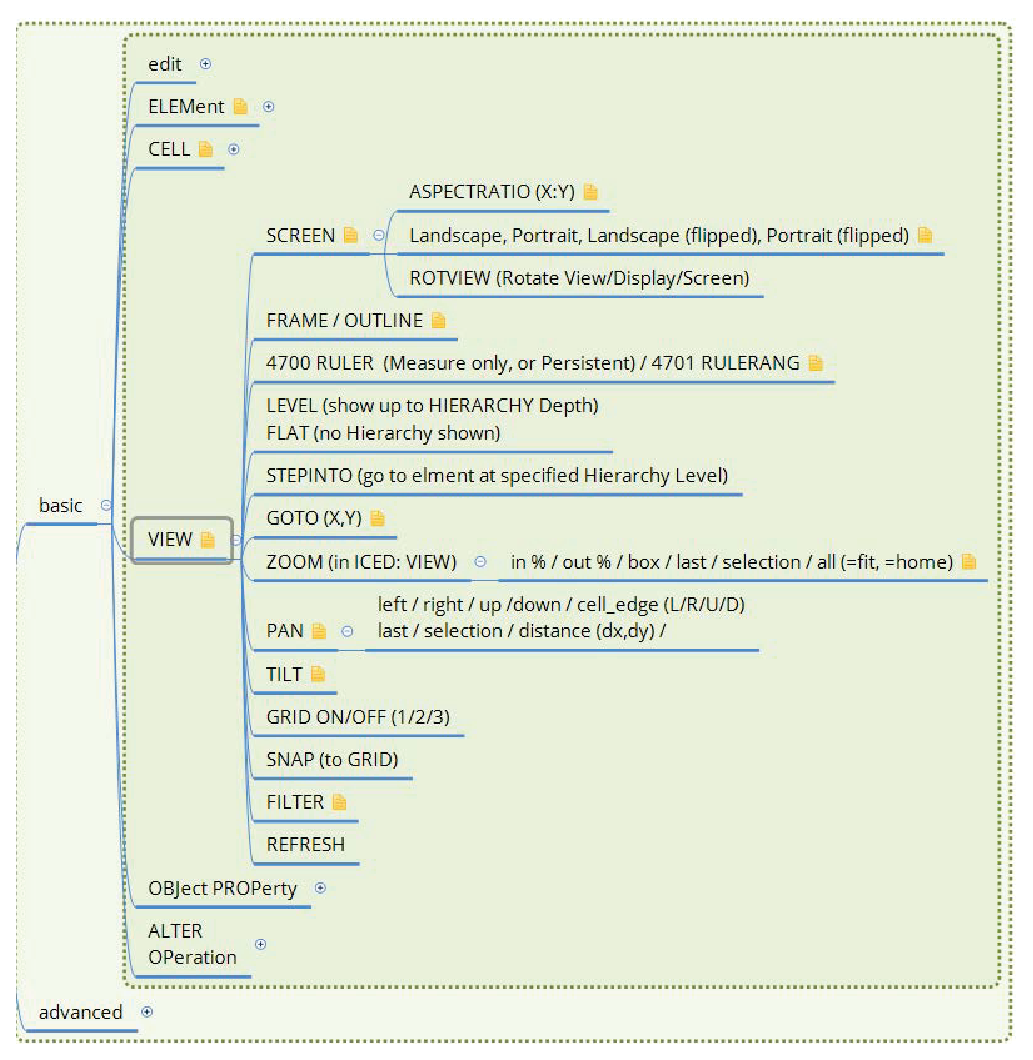
\includegraphics[width=4in]{./Layout/FigsCmd/CmdBasicView.eps}
	\caption{Commands to View Basic Elements 视图基本命令。}
	\label{FigCmdView}
\end{figure}
\subsubsection{屏幕设置(Screen)} \label{SectCmdViewScreen}
屏幕设置(Screen)调整屏幕的基本设置,比如纵宽比、页面设置、旋转设置。
\begin{itemize}
	\item Screen XtoY X Y  (设置屏幕纵宽比为X:Y)
	\item Screen Landscape (设置屏幕为横向)
	\item Screen Portrait  (设置屏幕为纵向)
	\item Screen Landscape flipped (设置屏幕为横向,左右颠倒)
	\item Screen Portrait  flipped (设置屏幕为纵向,上下颠倒)
	\item Screen Rotate    (设置屏幕旋转设定角度)
\end{itemize}

\subsubsection{边框显示(Frame/Outline)} \label{SectCmdViewFrame}
边框显示(Frame/Outline):显示或关闭基本图形和构元的边框
\begin{itemize}
	\item Frame On/Off   (显示或关闭基本图形和构元的边框)
	\item Outline On/Off (显示或关闭基本图形和构元的边框)
\end{itemize}

\subsubsection{标尺(Ruler)} \label{SectCmdViewRuler}
标尺(Ruler):显示或关闭测量的标尺。

RULER normally measures distance, but OptiMASK extents the ruler to angle measurement with 3 points, i.e., for consecutive 3 points A->B->C, the RULERANG tells the angle B.

支持厘米,毫米,英尺,英寸等多种刻度标尺。L-Edit use RULER as an annotation (which we defined in 4C01 NOTE)

\begin{itemize}
	\item Ruler On/Off   (显示或关闭测量的距离标尺)
	\item RulerAngle On/Off  (显示或关闭测量的角度标尺)
\end{itemize}

\subsubsection{层级深度(Level)} \label{SectCmdViewLevel}
层级(Level):显示构元引用层级深度(Hierarchy Level Depth)。程序可以设定最多层级256级,一般够用了。
\begin{itemize}
	\item View Level 1 to 10   (显示构元引用层级从第1级至第10级)
	\item View Flat 等同于 View Level 0 to 0  (显示所有构元列表,不分层级)
	\item GoTo Level 5 等同于 StepInto Level 5  (进入(激活)当前构元的子构元第5级)
\end{itemize}

\subsubsection{转至(GoTo)} \label{SectCmdViewGoTo}
转至(GoTo):转至指定的位置(Position)、构层(Layer)、构元(Cell)或者层级(Level)。
\begin{itemize}
	\item GoTo X Y   (转至指定的坐标位置(X,Y),即将此点设置为显示中心)
	\item GoTo Layer LAYERID/LAYERNAME (转至当前构元的指定构层)
	\item GoTo Cell  CELLID/CELLNAME (转至指定的构层)
	\item GoTo Level 5 (转至当前构元第5子级)
\end{itemize}

\subsubsection{缩放(Zoom)} \label{SectCmdViewZoom}
TILT, PAN, ZOOM are basic camera operations.

PAN -- Move Camera X or Y;

ZOOM -- Camera focus zoom in or out;

TILT -- Tilt the camera 

缩放(Zoom):缩放当前窗口的指定显示范围。缩放大小就用小数或者分数(包括$a/b$形式)表示。此处不用百分比符号\%,因为\%已经缺省允许为注释符号。
\begin{itemize}
	\item Zoom 0.80  (新视图是原视图的80\%,$<1$表示缩小)
	\item Zoom 1.20  (新视图是原视图的120\%,$>1$表示放大)
	\item Zoom in 1.20  (放大120\%,即新视图是原视图的120\%)
	\item Zoom out 1.20 (缩小120\%,即原视图是新视图的120\%)
	\item Zoom Box X0 Y0 X1 Y1  (新视图为矩形框选中的区域)
	\item Zoom Last  (转至上次的显示区域)
	\item Zoom Selection  (显示区域刚好包括所有选中的图元和构元)
	\item Zoom All  (显示区域显示当前构元的所有元素)
\end{itemize}

\subsubsection{平移(Pan)} \label{SectCmdViewPan}
平移(Pan):平移当前窗口的显示范围。平移时不改变显示的缩放。

When using keyboard <left>, <right>, <up>, <down>, the view change is panning. We allow command operation of panning as below:
\begin{itemize}
	\item Pan left/right/up/down  (显示范围左右上下移动1/4(缺省))
	\item Pan left/right/up/down 1/N (显示范围左右上下移动1/N,N为大于1的正整数)
	\item Pan cell (L/R/U/D)  (显示范围转至当前构元的左右上下边界)
	\item Pan Last  (转至上次的平移位置)
	\item Pan Selection  (移动至选中区域)
	\item Pan dX dY (显示中心移动(dX,dY))
\end{itemize}

\subsubsection{倾斜(Tilt)} \label{SectCmdViewTilt}
倾斜(Tilt):主要是3D图形时考虑,对于二维版图操作简单功能可以暂时不考虑。高级功能可以将二维版图操作倾斜指定视角。
\begin{itemize}
	\item Tilt AngleX AngleY AngleZ  (倾斜指定的(X,Y,Z)角度)
\end{itemize}

\subsubsection{格点(Grid)} \label{SectCmdViewGrid}
格点(Grid):显示或关闭显示屏上的格点。格点可以分多级(通常3或4级)。用户可任意定义每级格点的尺寸(缺省1/2/3/4级为1/0.1/0.01/0.001 user unit,比如\um)。
\begin{itemize}
	\item Grid On/Off   (显示或关闭显示屏上的各级格点)
	\item Grid 1/2/3/4 On/Off (显示或关闭显示屏上的指定级别的格点)
	\item Grid 4 Size 0.001 (第四级格点设置为0.001 user unit;其它级别类似设置)
\end{itemize}

\subsubsection{对格(Snap)} \label{SectCmdViewSnap}
对格(Snap): see \emph{ICED™ Command File Programmer's Reference}
\begin{verbatim} C:\icwin\doc\LAYOUT_PROGRAMMER_REF.PDF \end{verbatim} 

There are snap grid and snap angle parameters that control how you can digitize points with the cursor。

Coordinates in an ADD command will NOT be forced to lie on the resolution or
snap grids. When coordinates are digitized using the mouse, then you can be
sure that the coordinates are on the snap and resolution grids. However, if your
command file uses mathematical operations to calculate coordinates, they
probably do not lie on grid. You will need to perform extra processing to snap
the coordinates to grid before using them in an ADD command.

If you calculate coordinates, you should use the functions below to snap the
coordinates to grid. If you prefer to avoid rounding coordinates to grid, your
command file should check the value of the system macro RES.MODE to
determine if the user has set the resolution mode to "SOFT". If the resolution mode is "SOFT", then the decision is up to you.

However, if the resolution mode is "HARD" then the user has indicated that all
coordinates should be on grid.

The ROUND() function is usually used to round a coordinate pair to the nearest
point on the resolution grid. 

\subsubsection{过滤(Filter)} \label{SectCmdViewFltr}
过滤(Filter):只显示符合条件的图元或者构元。Advanced capability, not need in minimum version. Only show objects that satisfy the filter criteria. 
\begin{itemize}
	\item View Filter Show CellName Contain CHAR (仅显示构元名字包含指定字符的构元)
\end{itemize}

\subsubsection{刷新(Refresh)} \label{SectCmdViewRefresh}
刷新(Refresh):刷新当前视图。有时可能操作后,没有及时刷新显示,那么就强制用刷新(Refresh)命令重现显示。 
\begin{itemize}
	\item View Refresh (刷新当前视图显示)
\end{itemize}

\subsection{属性(Object Property))} \label{SectCmdProperty}

\subsection{变化(Alter)} \label{SectCmdCell}

\subsection{注意} \label{SectCmdNote} 
命令和脚本注意事项。

%%\pagestyle{empty}
%%\cleardoublepage
%%to generates one blank page for the next chapter to be on an odd page

%% Optimask Data Structure
%% Created: 2017-08-23; Updated: 2017-08-23;
%% by Henghua DENG, hdeng@optixera.com

\resetdatestamp %Date Stamp--Only use when custom package datestamp.sty is used.

%\part{Optimask Layout Design} \label{PartMaskDesign}
%本部分介绍Optimask版图设计软件基本框架,具体功能实现,主要界面,命令行及编程输入等等。

\chapter{Optimask Data Structure} \label{ChMaskDataStruct}
%======================================================================
%Heading Settings:
\markboth{Chapter~\thechapter.~Data~Structure}{} %\leftmark calls #1 parameter
%\markright{ } % new right header. Only used for two-side documents.

\pagestyle{fancy}
\fancyhead[RO,RE]{}
\fancyhead[LE]{\MakeUppercase{\leftmark}}
\fancyhead[LO]{\MakeUppercase{\rightmark}}
\fancyfoot[C]{\thepage}
%%\fancyfoot[L]{\today}

Optimask版图设计的数据结构(Data Structure)是非常重要的基本构架。Optimask版图数据结构基于GDSII格式,但是做了重要扩展为自定义格式。当版图Tape-Out时,自定义格式可以转换为标准GDSII格式。

%======================================================================
\section{Optimask数据结构基本构架} \label{SectDataStruct}
%======================================================================
Optimask数据结构基本构架其实很简单,主要分为基本图元(Element)和构元引用(Reference)两类。

\begin{figure}[htb!p] %h--here, t--top, b--bottom, p--page;
	\centering
	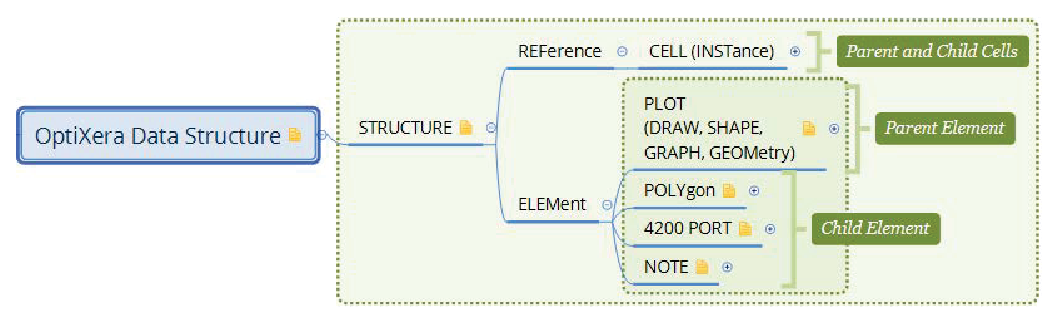
\includegraphics[width=4in]{./Layout/FigsData/Structure.eps}
	\caption{Optimask数据结构基本构架。}
	\label{FigDataStruct}
\end{figure}

%======================================================================
\section{Optimask基本图元(Element)数据结构} \label{SectDataElem}
%======================================================================
Optimask基本图元(Element)数据结构,包括绘制(Plot)、多边形(Polygon)、端口(Port)和标注(Note)。

基本图元(Element)是指所有尚没有组成构元结构的基本图形。GDSII格式主要包括矩形(Box), 多边形(Polygon), 线(Wire)等。其实所有的图形都可以转换为多边形(Polygon)。但是对于很多规则图形,直接存储为多边形比较占用空间。比如圆形,不管用多少个点近似为多边形,都不如直接存储圆心位置和半径大小准确和简洁。所以我们将基本图形稍微扩展出绘制(Plot)子结构。

基本图元(Element)之间的连接信息也经常需要用到。比如,对于光波导和微波波导等,经常需要确定光路和电磁波的路径。此时不同器件之间需要用端口(Port)来连接。

我们希望版图的理解和信息传递尽量有效,所以同时定义了标注(Note)来存储重要的设计信息。

\begin{figure}[htb!p] %h--here, t--top, b--bottom, p--page;
	\centering
	\subfigure[绘制(Plot)和多边形(Polygon)] {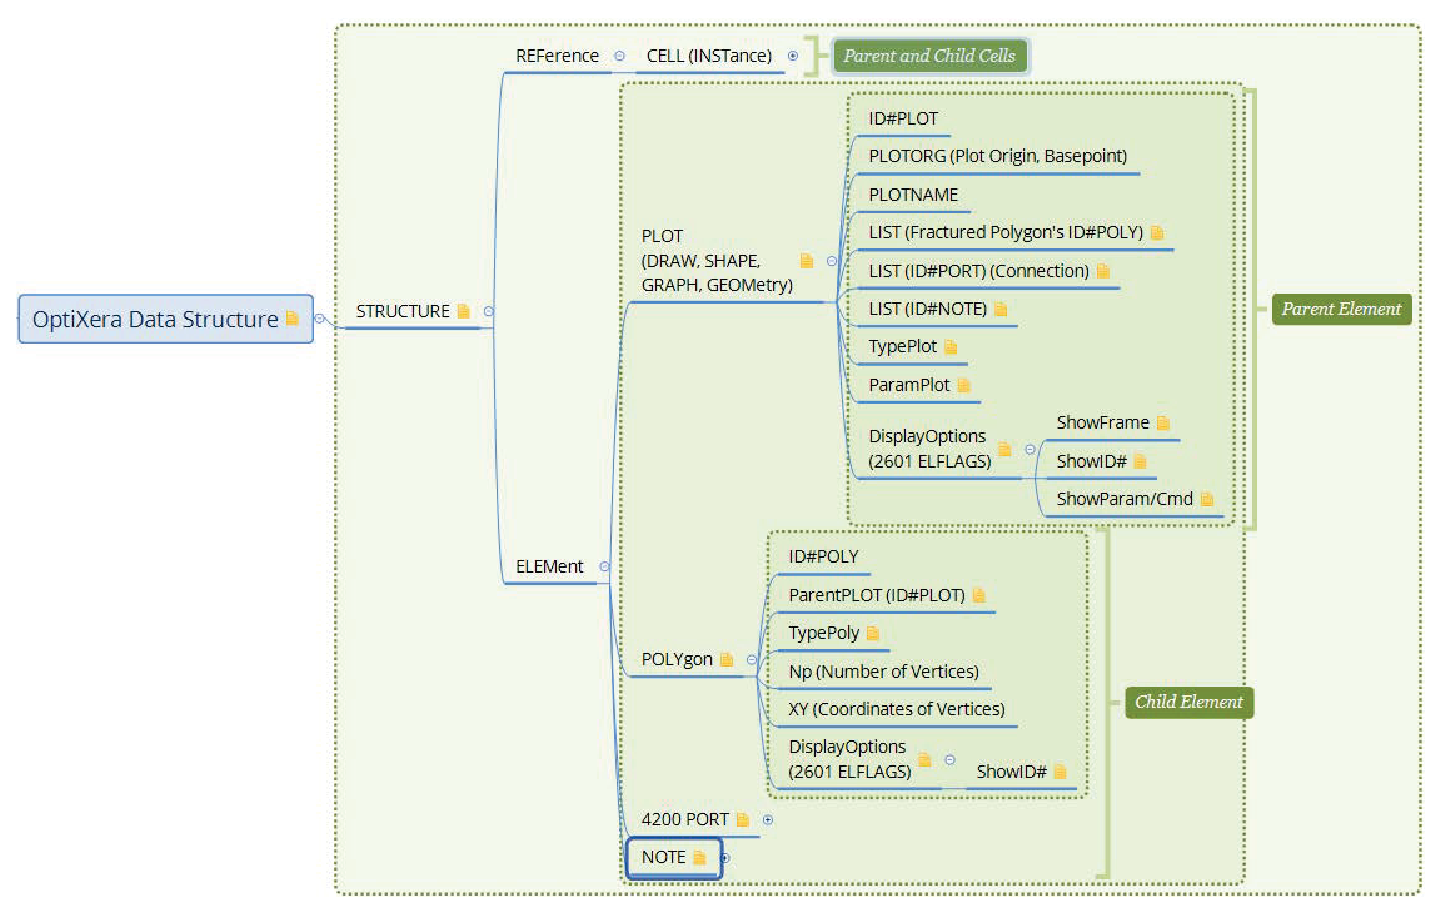
\includegraphics[width=3in]{./Layout/FigsData/ElemPlotPoly.eps}
		\label{FigDataElemPlotPoly}}
	\hfill
	\subfigure[端口(Port)和标注(Note)] {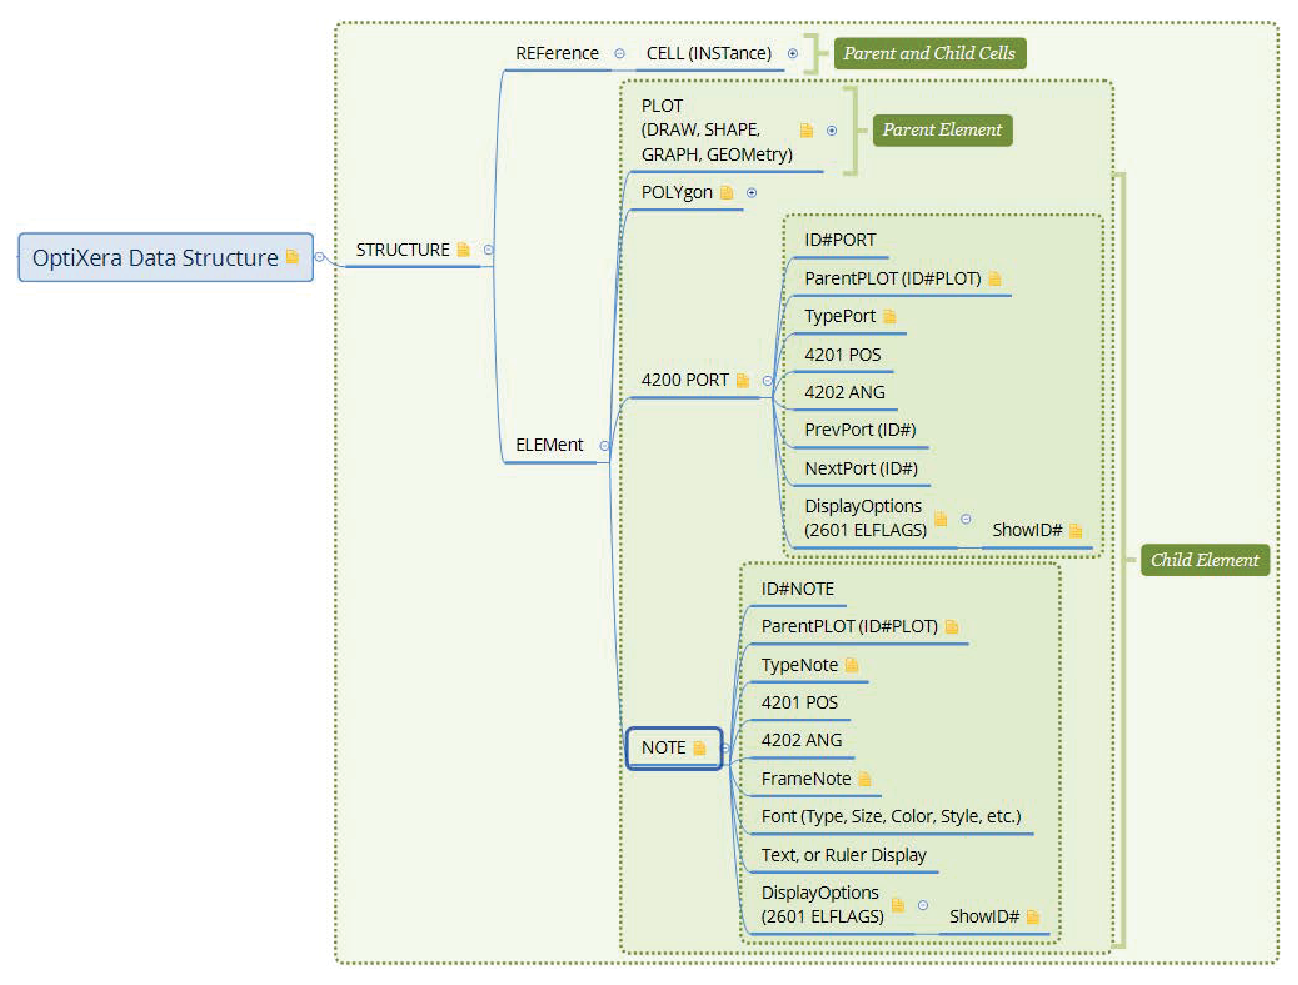
\includegraphics[width=3in]{./Layout/FigsData/ElemPortNote.eps}
		\label{FigDataElemPortNote}}
	\caption{Optimask基本图元(Element)数据结构,包括绘制、多边形、端口和注释。}
	\label{FigDataElem}
\end{figure}

\subsection{绘制(Plot)} \label{SectDataPlot} 
绘制(Plot)。

\subsection{多边形(Polygon)} \label{SectDataPoly} 
多边形(Polygon)。

\subsection{端口(Port)} \label{SectDataPort}
端口(Port)。

\subsection{标注(Note)} \label{SectDataNote} 
标注(Note)。

%======================================================================
\section{Optimask构元引用(Cell Reference)数据结构} \label{SectDataRef}
%======================================================================
Optimask构元引用(Cell Reference)数据结构。
\begin{figure}[htb!p] %h--here, t--top, b--bottom, p--page;
	\centering
	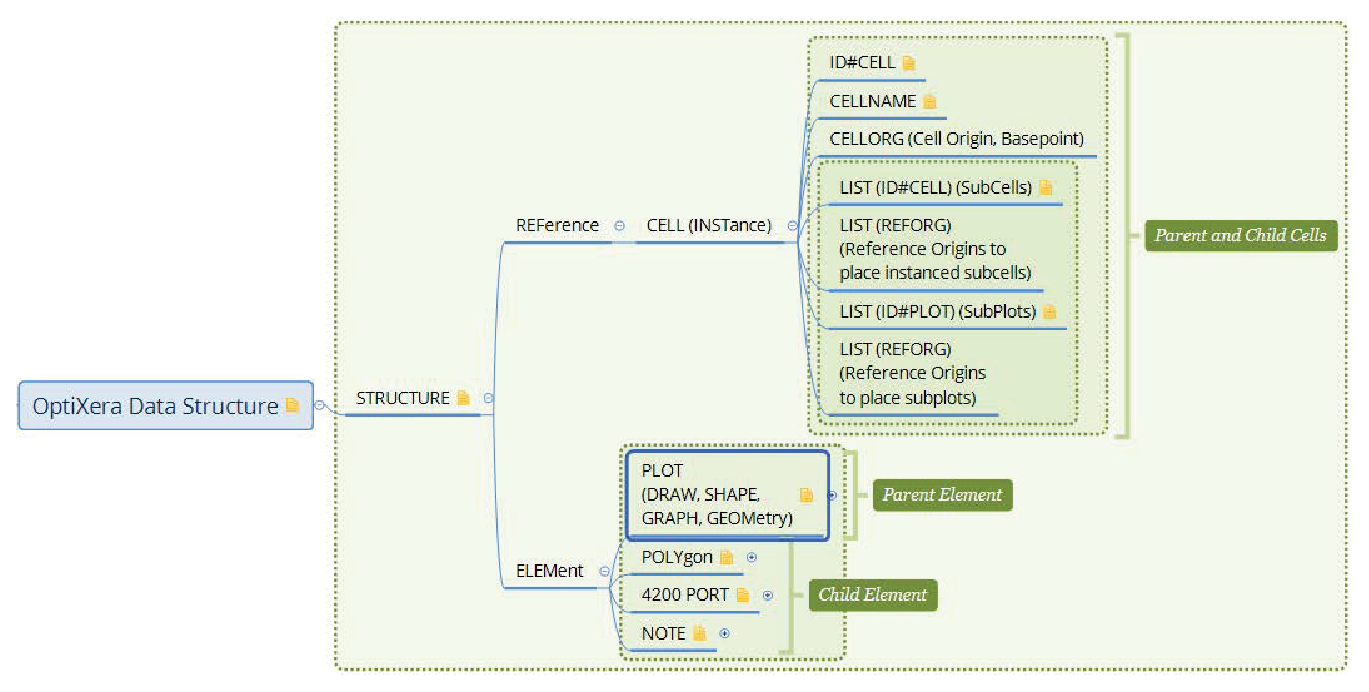
\includegraphics[width=4in]{./Layout/FigsData/RefCell.eps}
	\caption{Optimask构元引用(Cell Reference)数据结构。}
	\label{FigDataRef}
\end{figure}

%%\pagestyle{empty}
%%\cleardoublepage
%%to generates one blank page for the next chapter to be on an odd page


%%----------------------------------------------------------------------
%% Appendices
%%----------------------------------------------------------------------
%% Designate with \appendix declaration which just changes numbering style from here on
\appendix
%\include{./Apdx_CodeScript}

%----------------------------------------------------------------------
% Bibliography
%----------------------------------------------------------------------
% If done using the BibTeX program, use
%\bibliographystyle{plain} % sorted alphabetically, labeled with numbers
%\bibliography{keylatex} % names file keylatex.bib as my bibliography file
% OR, do it "by hand" inside a "thebibliography" environment
%%%%%%%%%%%%%%%%%%%%%%%%%%%
\bibliographystyle{IEEEtran}  %{IEEEtran.bst} %{IEEEtranS.bst} %plain, unsrt, abbrv, alpha
%\renewcommand\bibname{References} %\bibname for book-classes; %or \refname for article-classes.
\addcontentsline{toc}{chapter}{\bibname}

%\bibliography{../IEEE/IEEEabrv,../Deng,../AWG,../BOOK,../SIMU,../MGVI,../PRW,../SOI,../SPR,../THz}
%\bibliography{IEEEabrv,./biblib/AWG}
%\bibliography{IEEEabrv,./biblib/MMI}
%DO NOT INCLUDE FILE TYPE NAME!! %%NO SPACES BETWEEN DIFFERENT FILE NAMES!!

%----------------------------------------------------------------------
% END MATERIAL
%----------------------------------------------------------------------
% Glossary
% You could use a \begin{description} ... \end{description} for this
%\include{glossary}

% Index
% Put a \makeindex command in the Preamble if you use MakeIndex program
% and put
% \printindex % here
% OR, do it "by hand" inside \begin{theindex} ... \end{theindex}
%----------------------------------------------------------------------

%----------------------------------------------------------------------
% Curriculum Vitae %Optional
%----------------------------------------------------------------------

%----------------------------------------------------------------------

\end{document}
